% !TeX program = xelatex
% !TeX encoding = UTF-8 Unicode
% !BIB program = biber

\documentclass[ieee,english]{slides}

\DeclareMathOperator*{\argmax}{arg\,max}
\DeclareMathOperator*{\argmin}{arg\,min}
\newcommand{\norm}[1]{\left\lVert#1\right\rVert}

\title{Command Governor Supervisor Scheme Based On Region Of Attraction}

\addauthor{Álan Crístoffer e Sousa}{acristoffers@gmail.com}

\setorientador{Prof.\ Dr.\ Valter Júnior de Souza Leite}
\addcoorientador{Prof.\ Dr.\ Walter Lucia}

\addmembrobanca{Prof.\ Dr.\ Erivelton Geraldo Nepomuceno}
\addmembrobanca{Prof.\ Dr.\ Márcio Fantini Miranda}

\setdepartamento{Graduate Program in Electrical Engineering}
\seteixodeformacao{System Control}

\setlocal{Divinópolis}
\setano{2020}
\setmes{December}

\preamble{}

\addbibresource{bibliothek.bib}

\begin{document}
\maketitle{}

\begin{slide}{Index}
  \begin{minipage}[t][0.6\textheight][t]{0.5\textwidth}
    \tableofcontents[sections={1-3}]
  \end{minipage}
  \begin{minipage}[t][4\baselineskip][t]{0.5\textwidth}
    \tableofcontents[sections={4-}]
  \end{minipage}
  \vfill\null{}
\end{slide}

% !TeX root = document.tex
% !TeX encoding = UTF-8 Unicode

\section{Introduction}%
\label{sec:introduction}

\subsection{Switched Systems}%
\label{subsec:switched-systems}

\begin{slide}{Switched Systems}
  \begin{columns}[c]
    \begin{column}{0.48\textwidth}
      A switched system is a system composed of many subsystems, called modes,
      and a mode-transition rule.
    \end{column}%
    \hfill%
    \begin{column}{0.48\textwidth}
      \begin{equation}
        \begin{aligned}
          \dot{x}(t) & = f_{\sigma(t)}(t,x(t),u(t)), \\
          y(t)       & = g_{\sigma(t)}(t,x(t)),
        \end{aligned}
      \end{equation}
      \vspace*{1cm}
      \begin{equation}
        \begin{aligned}
          \dot{x}(t) & = A_{\sigma(t)}x(t) + B_{\sigma(t)}u(t), \\
          y(t)       & = C_{\sigma(t)}x(t) + D_{\sigma(t)}u(t).
        \end{aligned}
      \end{equation}
    \end{column}%
  \end{columns}
\end{slide}

\begin{slide}{Switched Systems Stability Problem}
  \begin{columns}[c]
    \begin{column}{0.48\textwidth}
      The system is stable under arbitrary switching if\\
      \vspace*{1cm}
      This stability guarantee is only valid inside the region
    \end{column}%
    \hfill%
    \begin{column}{0.48\textwidth}
      \begin{equation}
        A_{i}^{\top}P+PA_{i} \prec{} 0.
      \end{equation}
      \vspace*{1cm}
      \begin{equation}
        x^{\top}Px \leq 1
      \end{equation}
    \end{column}%
  \end{columns}
\end{slide}

\subsection{Command Governor}%
\label{subsec:cg}

\begin{slide}{Problem Description}
  \begin{columns}[c]
    \begin{column}{0.48\textwidth}
      How to keep the system's state and/or inputs constrained.
    \end{column}%
    \hfill%
    \begin{column}{0.48\textwidth}
      \begin{figure}[ht!]
  \centering
  \captionsetup{justification=centering}
  \begin{tikzpicture}[auto,node distance=1cm,>={Stealth},waypoint/.style={circle,inner sep=0pt,outer sep=0pt,thick},state/.style={circle,minimum size=1em,inner sep=0pt,outer sep=0pt},constraint/.style={ellipse,fill opacity=0.7,text opacity=1}]
    \node (x)  [state]                {\(\star\)};
    \node (w1) [waypoint,below=of x]  {};
    \node (w2) [waypoint,above=of x]  {};
    \node (w3) [waypoint,left=of x]  {};
    \node (a0) [waypoint,below left=3cm of x]   {};
    \node (a1) [waypoint,right=4cm of a0] {};
    \node (a2) [waypoint,above=4cm of a0] {};

    \begin{scope}[on background layer]
      \node (c1) [constraint,fill=cyan!80,fit=(w1) (w2) (w3)]    {};
    \end{scope}

    \draw [->] (a0) -- node [below] {\(x_{1}\)} (a1);
    \draw [->] (a0) -- node [left]  {\(x_{2}\)} (a2);
  \end{tikzpicture}%
  \caption{Constraint region and system's state}%
  \label{fig:dt-example}
\end{figure}

    \end{column}%
  \end{columns}
\end{slide}

\begin{slide}{Command Governor}
  \begin{columns}[c]
    \begin{column}{0.55\textwidth}
      % !TeX root = ../document.tex
% !TeX encoding = UTF-8 Unicode

\begin{figure}[ht!]
  \centering
  \captionsetup{justification=centering}
  % \resizebox{0.8\linewidth}{!}{%
  \begin{tikzpicture}[node distance=1cm,block/.style={align=center,draw,shape=rectangle,very thick,minimum height=2em, minimum width=3em},>={Stealth}]

    \node (r)  []                      {\(r(k)\)};
    \node (cg) [block, right=of r]     {Command\\Governor};
    \node (C)  [block, right=of cg]    {Primal\\Controller};
    \node (G)  [block, right=of C]     {System};
    \node (y)  [right=of G.north east] {\(y(k)\)};
    \node (c)  [right=of G.south east] {\(c(k)\)};
    \node (e)  [below=of C]            {\(\begin{bmatrix}x_{c}(k)\\x(k)\end{bmatrix}\)};
    \node [draw=blue,rectangle,dashed,fit=(C) (G) (e)] {};

    \draw [->, thick] (r) -- (cg);
    \draw [->, thick] (cg) -- node [above] {\(g(k)\)} (C);
    \draw [->, thick] (C) -- node (u) [above] {\(u(k)\)} (G);

    \draw [->, thick] ([yshift=-3mm]G.north east) -- (y.west);
    \draw [->, thick] ([yshift=3mm]G.south east) -- (c.west);
    \draw [->, thick] (G) |- node (x) [near start, above right] {\(x(k)\)} ([yshift=1em]e.south east);
    \draw [->, thick] (x) -| ([xshift=5mm]C.south);
    \draw [->, thick] (C) -- node [left] {\(x_{c}(k)\)} (e.north);
    \draw [->, thick] (e.west) -| (cg.south);
  \end{tikzpicture}%
  % }
  \caption{Command Governor Block Diagram.}%
  \label{fig:cg-schematic}
\end{figure}

    \end{column}%
    \hfill%
    \begin{column}{0.45\textwidth}
      \vspace*{0.5cm}
      \begin{equation}
        \begin{aligned}
          x(k+1) & = A_{i}x(k)+B_{i}u(k), \\
          y(k)   & = C_{i}x(k)+D_{i}u(k), \\
          c(k)   & = E_{i}x(k)+F_{i}u(k).
        \end{aligned}
      \end{equation}
      \begin{enumerate}
        \item \(\mathcal{C}\) is the set of restrictions.
        \item \(\mathcal{W} = \{\omega\in\mathbb{R}^{n_y}: c(k)\in\mathcal{C},k\rightarrow\infty{}\}.\)
        \item \(\mathcal{V}(x(k))=\{\omega\in\mathcal{W}:c(k)\in\mathcal{C},0<k\leq{}k_0\}.\)
      \end{enumerate}
      \vspace*{0.5cm}
      \begin{equation}
        \begin{aligned}
          g(k)=\argmin_{\omega\in\mathcal{V}(x(k))} & \norm{\omega-r(k)}^2_\Psi
        \end{aligned}
      \end{equation}
    \end{column}%
  \end{columns}
\end{slide}

\subsection{Supervisor}%
\label{subsec:supervisor}

\begin{slide}{Supervisor}
  \begin{figure}[ht!]
  \centering
  \captionsetup{justification=centering}
  \resizebox{!}{0.7\textheight}{%
    \begin{tikzpicture}[auto,node distance=1cm,>={Stealth},block/.style={draw,rectangle,minimum height=2em,minimum width=4em,thick},sum/.style={draw,circle,thick},point/.style={coordinate},dot/.style={draw,thick,circle,minimum size=0.5em},tight/.style={inner sep=0pt,outer sep=0pt}]
      \node (cg2) [block]              {\(CG_{2}\)};
      \node (C2)  [block,right=of cg2] {\(PC_{2}\)};
      \node (X2)  [tight,below=of C2]  {\(\begin{bmatrix}x_{C2}(k)\\x(k)\end{bmatrix}\)};
      \node [draw,rectangle,dashed,fit=(cg2) (C2) (X2)] {};
      \draw [->,thick] (cg2) -> node [below] {\(g_{2}(k)\)} (C2);
      \draw [->,thick] (C2) -> node [swap] {\(x_{C2}(k)\)} (X2);
      \draw [->,thick] (X2) -| (cg2);

      \node (cg3) [block,above=3cm of cg2] {\(CG_{3}\)};
      \node (C3)  [block,right=of cg3]     {\(PC_{3}\)};
      \node (X3)  [tight,below=of C3]      {\(\begin{bmatrix}x_{C3}(k)\\x(k)\end{bmatrix}\)};
      \node [draw,rectangle,dashed,fit=(cg3) (C3) (X3)] {};
      \draw [->,thick] (cg3) -> node [below] {\(g_{3}(k)\)} (C3);
      \draw [->,thick] (C3) -> node [swap] {\(x_{C3}(k)\)} (X3);
      \draw [->,thick] (X3) -| (cg3);

      \node (supervisor) [block,above left=of cg3,draw=orange] {Supervisor};
      \node (r) [left=of supervisor] {\(r(k)\)};
      \draw [->,thick] (supervisor) |- (cg2);
      \draw [->,thick] (supervisor) |- (cg3);

      \node (sw1) [tight,dot,right=2cm of C2]          {};
      \node (sw2) [tight,dot,above right=0.5em of sw1] {};
      \node (sw3) [tight,dot,below right=0.5em of sw1] {};
      \node (sw4) [point,right=1em of sw1]             {};
      \node (sw5) [point,right=1em of sw4]             {};
      \node (switch) [draw,rectangle,tight,fit=(sw1) (sw2) (sw3) (sw5),thick] {};
      \draw [thick] (sw5) -- (sw4) -- (sw2);

      \node (system) [block,right=1.5cm of switch] {System};
      \node (y) [right=of system] {\(y(k)\)};

      \draw [->,thick] (r) |- (supervisor);
      \draw [->,thick,dotted,draw=orange] ([yshift=0.75em]supervisor.south east) -| ([xshift=-0.5em]switch.north east);
      \draw [->,thick] (system) -- (y);
      \draw [->,thick,draw=blue] (switch) -- node {\(u_{i}(k)\)} (system);
      \draw [->,thick,draw=blue] (C3.east) -| node [below left] {\(u_{3}(k)\)} (sw2.north);
      \draw [->,thick,draw=blue] (C2.east) --  node {\(u_{2}(k)\)} (sw1.west);
      \draw [->,thick,draw=red] (system) |- node [above left] {\(x(k)\)} ([yshift=0.75em]X2.south east);
      \draw [->,thick,draw=red] (system) |- node [above left] {\(x(k)\)} ([yshift=0.75em]X3.south east);
      \draw [->,thick,draw=red] (system) |- ([yshift=-0.75em]supervisor.north east);
      \draw [->,thick,draw=red] (system) |- ++(-1cm,-1cm) -| ([xshift=-1em]C2.south east);
      \draw [->,thick,draw=red] (system) |- ++(-1cm,3cm)  -| ([xshift=-1em]C3.south east);
    \end{tikzpicture}%
  }%
  \caption{Supervisor Block Diagram.}%
  \label{fig:supervisor-schematic}
\end{figure}

\end{slide}

\subsection{Region of Attraction}%
\label{subsec:roa}

\begin{slide}{Poincaré-Bendixson's Theorem}
  \begin{figure}[!htb]
    \centering
    %
    \begin{subfigure}[b]{0.45\linewidth}
      \centering
      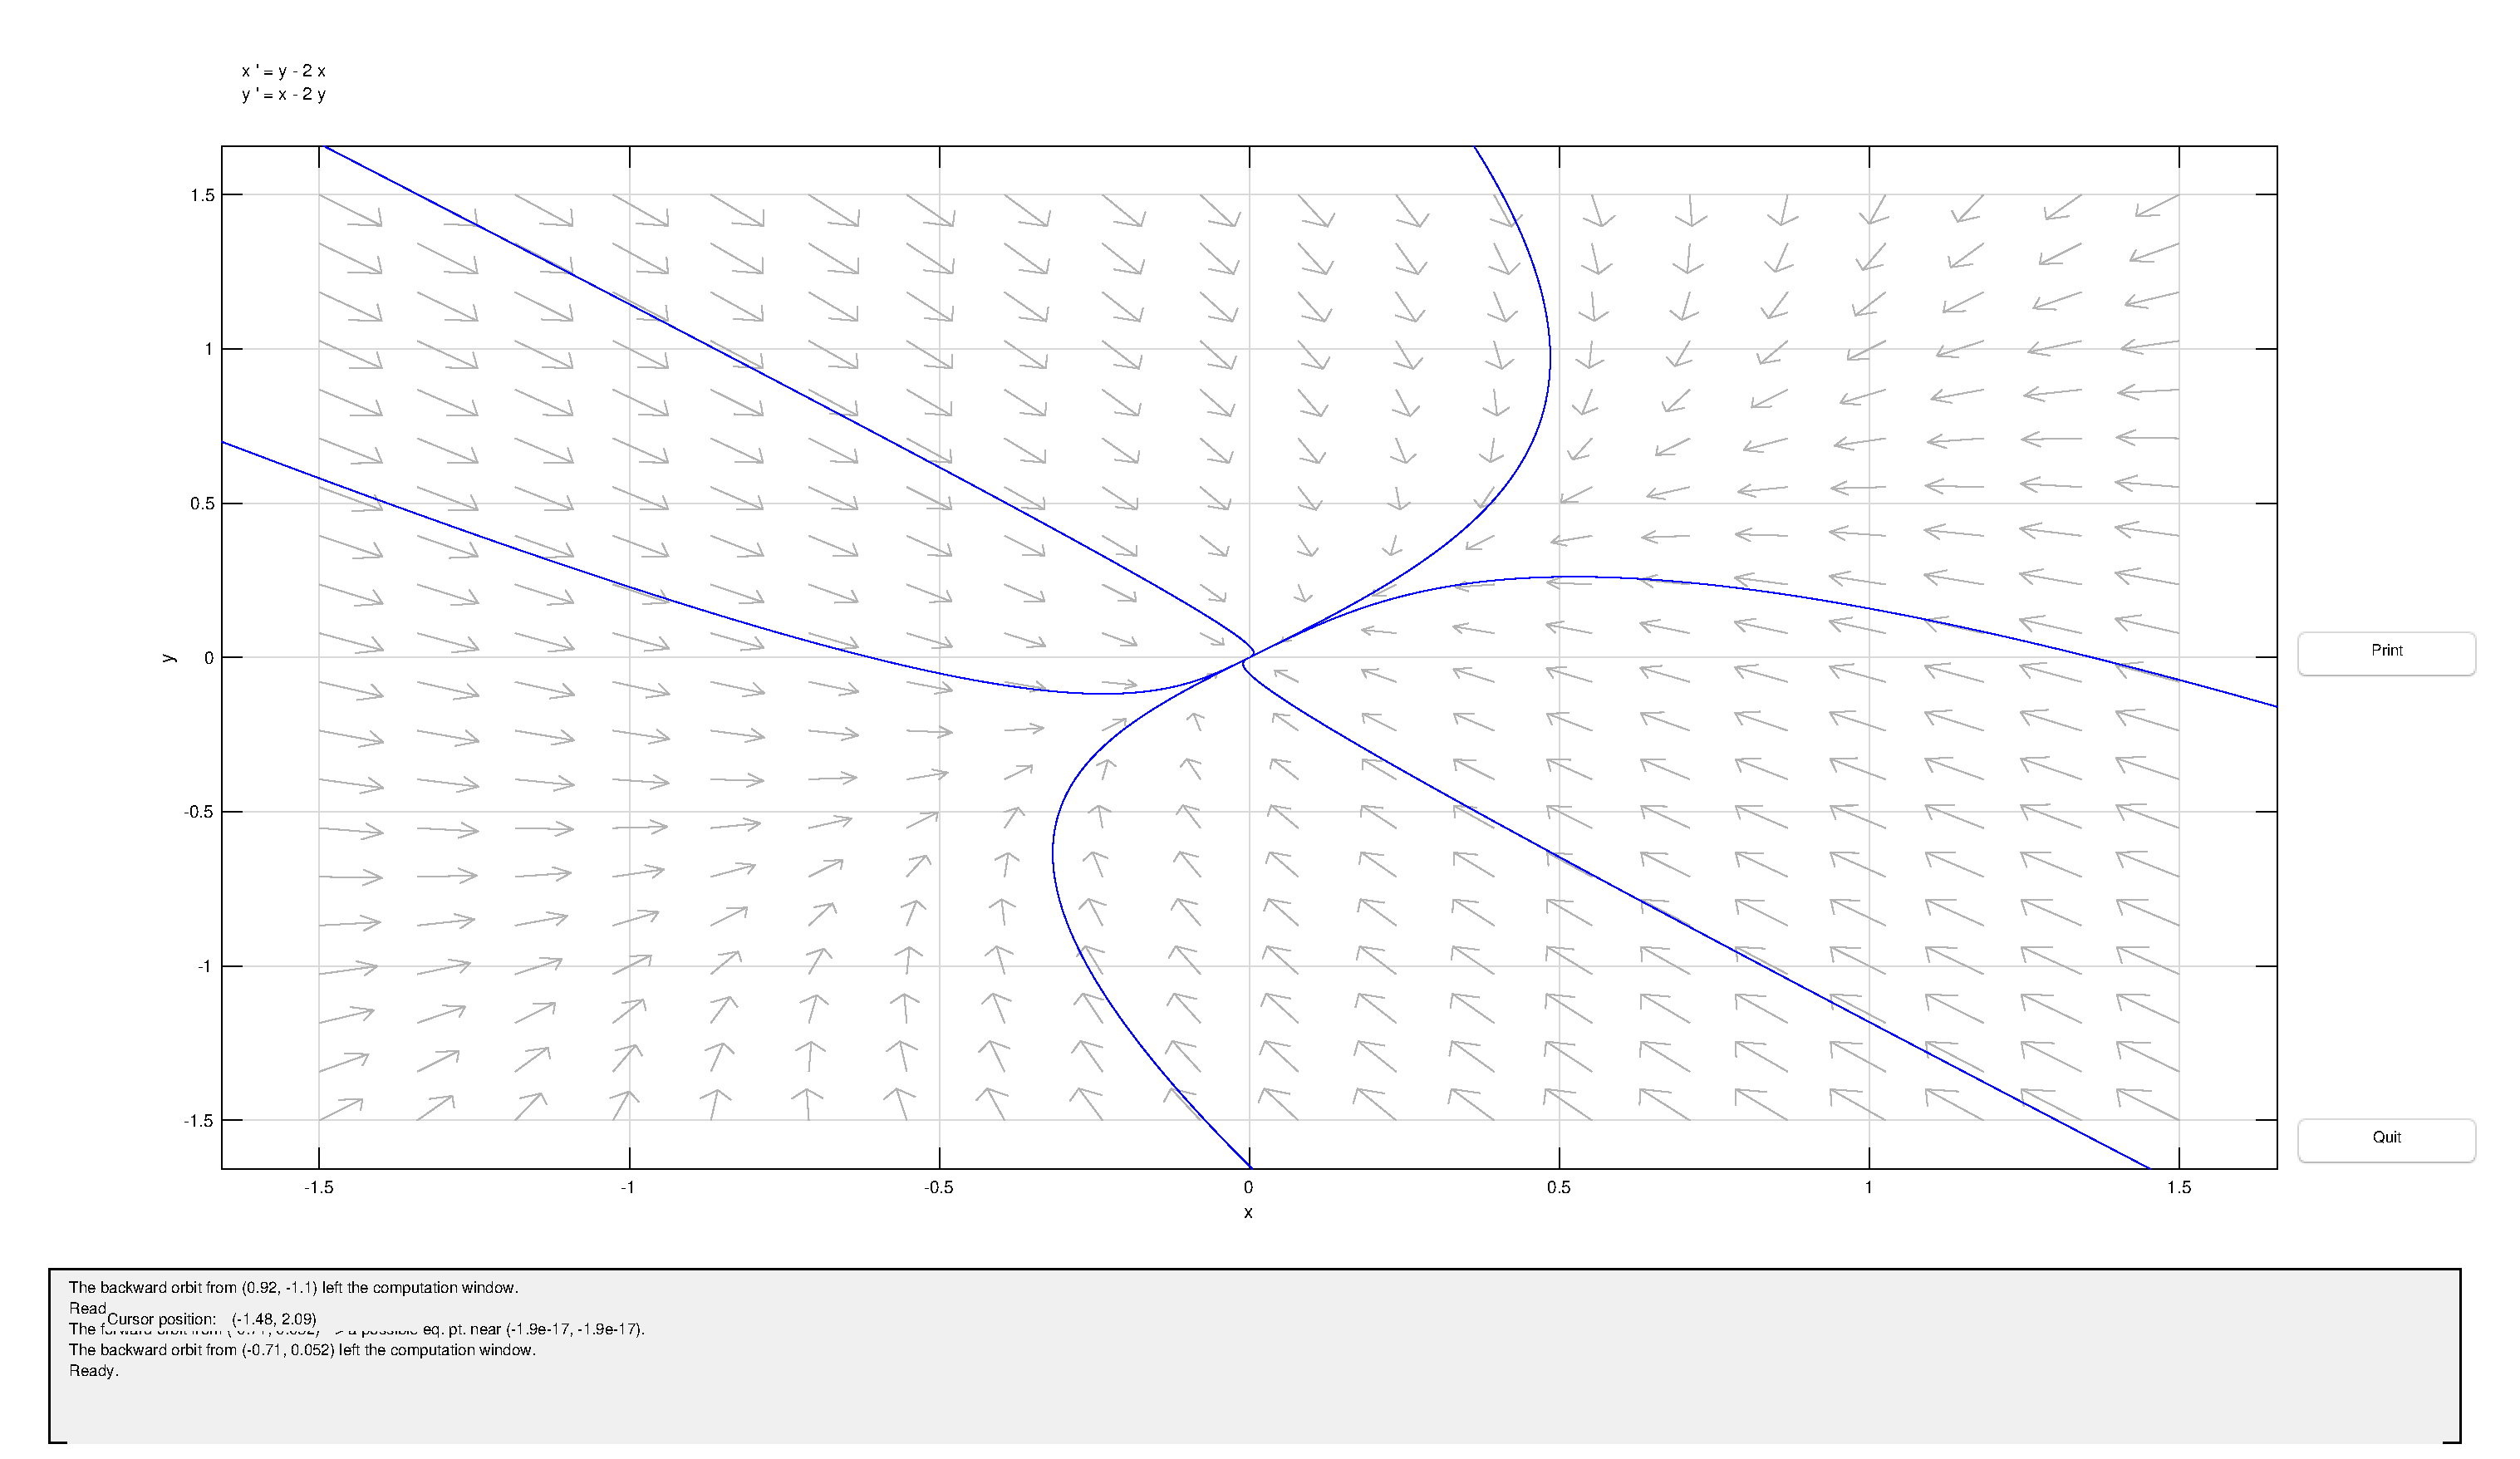
\includegraphics[trim=116 155 125 55,clip,width=\linewidth]{imgs/stable-point}
      \caption{Stable point}%
      \label{fig:stable-point}
    \end{subfigure}
    %
    \begin{subfigure}[b]{0.45\linewidth}
      \centering
      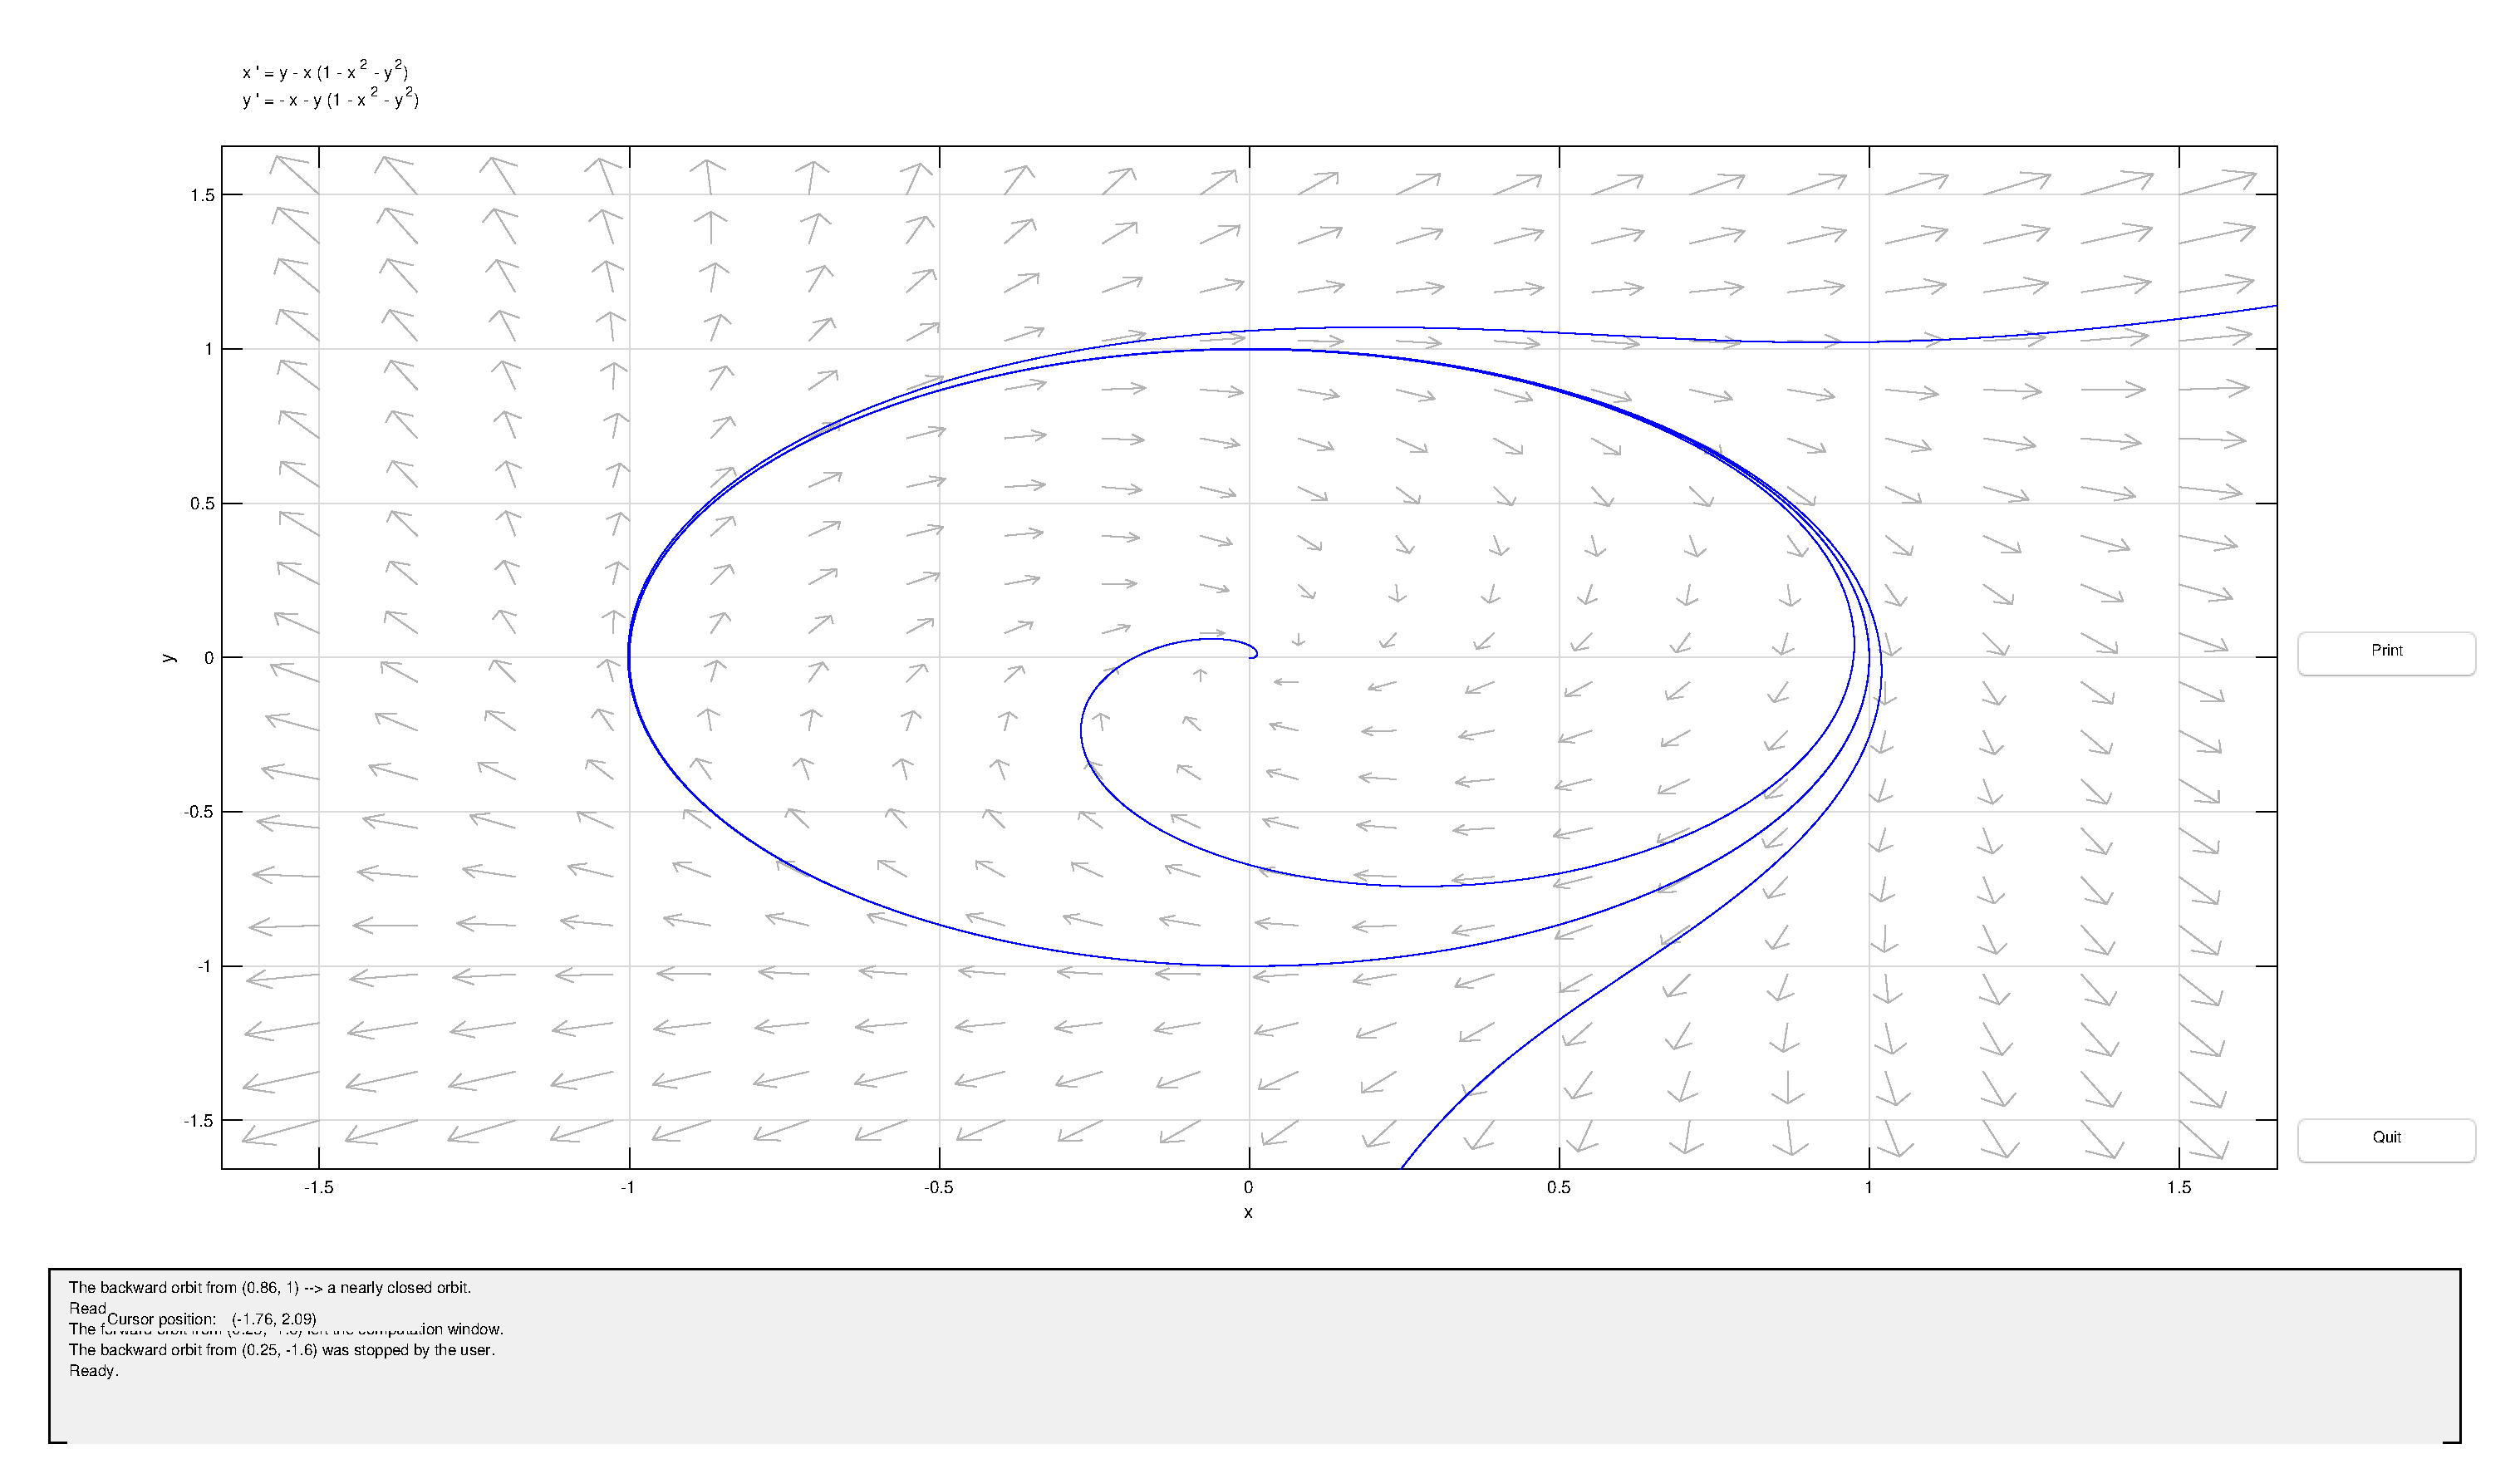
\includegraphics[trim=116 155 125 55,clip,width=\linewidth]{imgs/semi-stable-cycle}
      \caption{Semi-stable cycle}%
      \label{fig:semi-stable-cycle}
    \end{subfigure}
    %
    \caption{Different cycles' gradient maps}%
    \label{fig:poincare-cycles}
  \end{figure}
  \begin{equation}
    \nabla{}H(x)f(x) \leq 0
  \end{equation}
\end{slide}

\begin{slide}{Lyapunov's Theorem}
  \begin{equation}
    \begin{aligned}
      V(x)       & = 0 \iff x = 0,                                       \\
      V(x)       & > 0 \iff x \ne 0,                                     \\
      V(x_{1})   & > V(x_{2}) \iff x_{1} > x_{2}                         \\
      \dot{V}(x) & = \nabla{}V(x)f(x) \le 0 \phantom{0} \forall x \ne 0,
    \end{aligned}
  \end{equation}
\end{slide}

% !TeX root = document.tex
% !TeX encoding = UTF-8 Unicode

\section{Switching Rules}%
\label{sec:switching-rules}

\subsection{Dwell-time}%
\label{subsec:dwell-time}

\begin{slide}{Dwell-time}
  \begin{columns}[c]
    \begin{column}{0.48\textwidth}
      The system must wait \(T\) seconds before switching modes.
      \begin{equation}
        \mathcal{D}_{T} := \{\sigma(\cdot):t_{k+1}-t_{k}\ge{}T\}.
      \end{equation}
    \end{column}%
    \hfill%
    \begin{column}{0.48\textwidth}
      \begin{figure}[ht!]
  \centering
  \captionsetup{justification=centering}
  \begin{tikzpicture}[auto,node distance=3cm,>={Stealth},waypoint/.style={draw,circle,minimum size=1em,inner sep=0pt,outer sep=0pt,thick},state/.style={draw,thick,circle,minimum size=1em,inner sep=0pt,outer sep=0pt},constraint/.style={ellipse,fill opacity=0.7,text opacity=1}]
    \node (x)  [state]                {\(\bullet\)};
    \node (w1) [waypoint,below=of x]  {\(\diamond\)};
    \node (w2) [waypoint,right=of w1] {\(\diamond\)};
    \node (w3) [waypoint,above=of w2] {\(\star\)};

    \begin{scope}[on background layer]
      \node (c1) [constraint,fill=cyan!80,fit=(x) (w1)]    {};
      \node (c2) [constraint,fill=green!80,fit=(w1) (w2)]  {};
      \node (c3) [constraint,fill=orange!80,fit=(w2) (w3)] {};
    \end{scope}

    \draw [->,thick] (x) -- (w1);
    \draw [->,thick] (w1) -- (w2);
    \draw [->,thick] (w2) -- (w3);
  \end{tikzpicture}%
  \caption{Dwell-time illustrative example}
\end{figure}

    \end{column}%
  \end{columns}
\end{slide}

\subsection{Region of Attraction}%
\label{subsec:roa-rule}

\begin{slide}{Region of Attraction}
  \begin{columns}[c]
    \begin{column}{0.48\textwidth}
      \begin{itemize}
        \item The region of attraction guarantees the stability after switching;
        \item an optional, hybrid switch can be used.
      \end{itemize}
    \end{column}%
    \hfill%
    \begin{column}{0.48\textwidth}
      \begin{figure}[ht!]
  \centering
  \captionsetup{justification=centering}
  \begin{tikzpicture}[auto,node distance=2cm,>={Stealth},waypoint/.style={draw,circle,minimum size=1em,inner sep=0pt,outer sep=0pt,thick},state/.style={draw,thick,circle,minimum size=1em,inner sep=0pt,outer sep=0pt},constraint/.style={ellipse,fill opacity=0.7,text opacity=1}]
    \node (x)  [state]                {\(\bullet\)};
    \node (w1) [waypoint,below=of x]  {\(\diamond\)};
    \node (w2) [waypoint,right=of w1] {\(\diamond\)};
    \node (w3) [waypoint,above=of w2] {\(\star\)};

    \begin{pgfonlayer}{background}
      \node (c1) [name path=c1,constraint,fill=cyan!80,fit=(x) (w1)]    {};
      \node (c2) [name path=c2,constraint,fill=green!80,fit=(w1) (w2)]  {};
      \node (c3) [name path=c3,constraint,fill=orange!80,fit=(w2) (w3)] {};
    \end{pgfonlayer}

    \node (roa1) [circle,very thick,draw=cyan!80,dashed,fit=(c1)]   {};
    \node (roa2) [circle,very thick,draw=green!80,dashed,fit=(c2)]  {};
    \node (roa3) [circle,very thick,draw=orange!80,dashed,fit=(c3)] {};

    \coordinate (i11) at (intersection of w1--x and roa2);
    \path[name path=xw1] (x)--(w1);
    \path[name intersections={of=xw1 and c2,by=i12}];

    \coordinate (i21) at (intersection of w2--w1 and roa3);
    \path[name path=xw2] (w1)--(w2);
    \path[name intersections={of=xw2 and c3,by=i22}];

    \draw [->,thick]        (x) -- (i11);
    \draw [->,thick,dashed] (i11) -- (i12);
    \draw [->,thick]        (i12) -- (i21);
    \draw [->,thick,dashed] (i21) -- (i22);
    \draw [->,thick]        (i22) -- (w3);
  \end{tikzpicture}%
  \caption{Region of attraction illustrative example}%
  \label{fig:roa-example}
\end{figure}

    \end{column}%
  \end{columns}
\end{slide}

% !TeX root = document.tex
% !TeX encoding = UTF-8 Unicode

\section{Results}%
\label{sec:results}

\subsection{Level System}%
\label{subsec:level-system}

\begin{slide}{System Description}
  \begin{figure}[ht!]
    \centering
    \captionsetup{justification=centering}
    \tikzset{every picture/.style={line width=0.75pt}}
    \resizebox{!}{0.75\textheight}{%
        \tikzset{every picture/.style={line width=0.75pt}} %set default line width to 0.75pt        
    \begin{tikzpicture}[x=0.75pt,y=0.75pt,yscale=-1,xscale=1]
        %uncomment if require: \path (0,459); %set diagram left start at 0, and has height of 459
        %Straight Lines [id:da5688929335924803] 
        \draw    (310.5,121) -- (310.5,341) -- (171,342) -- (170,121) ;
        %Straight Lines [id:da5444294116492245] 
        \draw    (530,120) -- (530,340) -- (390.5,341) -- (389.5,120) ;
        %Straight Lines [id:da5805131124126722] 
        \draw    (200,360) -- (200,398) ;
        \draw [shift={(200,400)}, rotate = 270] [color={rgb, 255:red, 0; green, 0; blue, 0 }  ][line width=0.75]    (10.93,-3.29) .. controls (6.95,-1.4) and (3.31,-0.3) .. (0,0) .. controls (3.31,0.3) and (6.95,1.4) .. (10.93,3.29)   ;
        %Straight Lines [id:da36945578968673487] 
        \draw    (510,360) -- (510,398) ;
        \draw [shift={(510,400)}, rotate = 270] [color={rgb, 255:red, 0; green, 0; blue, 0 }  ][line width=0.75]    (10.93,-3.29) .. controls (6.95,-1.4) and (3.31,-0.3) .. (0,0) .. controls (3.31,0.3) and (6.95,1.4) .. (10.93,3.29)   ;
        %Straight Lines [id:da3077937138084411] 
        \draw    (310,300) -- (340,300) ;
        %Straight Lines [id:da6773172185122848] 
        \draw    (310,320) -- (340,320) ;
        %Shape: Rectangle [id:dp35476624369345366] 
        \draw   (340,290) -- (360,290) -- (360,330) -- (340,330) -- cycle ;
        %Straight Lines [id:da9030142425581202] 
        \draw    (360,300) -- (390,300) ;
        %Straight Lines [id:da9329287059080266] 
        \draw    (360,320) -- (390,320) ;
        %Straight Lines [id:da7833363422326105] 
        \draw    (340,290) -- (360,330) ;
        %Straight Lines [id:da26540765973372593] 
        \draw    (360,290) -- (340,330) ;
        %Straight Lines [id:da7238601427391023] 
        \draw    (470.02,340) -- (470,370) ;
        %Straight Lines [id:da21192498383993508] 
        \draw    (450.02,339.99) -- (450,369.99) ;
        %Shape: Rectangle [id:dp4746471043409347] 
        \draw   (480,370.01) -- (479.99,390.01) -- (439.99,389.98) -- (440,369.98) -- cycle ;
        %Straight Lines [id:da6336671048955647] 
        \draw    (470,389.99) -- (469.98,400) ;
        %Straight Lines [id:da6700066277567417] 
        \draw    (450,389.99) -- (449.98,400) ;
        %Straight Lines [id:da928718960478936] 
        \draw    (480,370.01) -- (439.99,389.98) ;
        %Straight Lines [id:da1540497075962557] 
        \draw    (479.99,390.01) -- (440,369.98) ;
        %Straight Lines [id:da7575667165517417] 
        \draw    (240.03,340.01) -- (240.01,370.01) ;
        %Straight Lines [id:da24987185404211631] 
        \draw    (220.03,340) -- (220.01,370) ;
        %Shape: Rectangle [id:dp2771887371908066] 
        \draw   (250.01,370.02) -- (250,390.02) -- (210,389.99) -- (210.01,369.99) -- cycle ;
        %Straight Lines [id:da9912034440398235] 
        \draw    (240,390) -- (240,400) ;
        %Straight Lines [id:da11904000202181764] 
        \draw    (220,390) -- (220,400) ;
        %Straight Lines [id:da7480508238760858] 
        \draw    (250.01,370.02) -- (210,389.99) ;
        %Straight Lines [id:da7049908339863217] 
        \draw    (250,390.02) -- (210.01,369.99) ;
        %Straight Lines [id:da9101133488343268] 
        \draw    (240,120) -- (240,158) ;
        \draw [shift={(240,160)}, rotate = 270] [color={rgb, 255:red, 0; green, 0; blue, 0 }  ][line width=0.75]    (10.93,-3.29) .. controls (6.95,-1.4) and (3.31,-0.3) .. (0,0) .. controls (3.31,0.3) and (6.95,1.4) .. (10.93,3.29)   ;
        %Straight Lines [id:da11474588029910615] 
        \draw    (460,120) -- (460,158) ;
        \draw [shift={(460,160)}, rotate = 270] [color={rgb, 255:red, 0; green, 0; blue, 0 }  ][line width=0.75]    (10.93,-3.29) .. controls (6.95,-1.4) and (3.31,-0.3) .. (0,0) .. controls (3.31,0.3) and (6.95,1.4) .. (10.93,3.29)   ;
        %Curve Lines [id:da10596831311641142] 
        \draw    (170,200) .. controls (210,170) and (270,230) .. (310,200) ;
        %Curve Lines [id:da32042097611565956] 
        \draw    (390,250) .. controls (430,220) and (490,280) .. (530,250) ;
        %Curve Lines [id:da9628648357071894] 
        \draw  [dash pattern={on 0.84pt off 2.51pt}]  (170,250) .. controls (210,220) and (270,280) .. (310,250) ;
        %Curve Lines [id:da13605436176729158] 
        \draw  [dash pattern={on 0.84pt off 2.51pt}]  (390,200) .. controls (430,170) and (490,230) .. (530,200) ;
        %Straight Lines [id:da6375240487876032] 
        \draw    (140,202) -- (140,338) ;
        \draw [shift={(140,340)}, rotate = 270] [fill={rgb, 255:red, 0; green, 0; blue, 0 }  ][line width=0.75]  [draw opacity=0] (8.93,-4.29) -- (0,0) -- (8.93,4.29) -- cycle    ;
        \draw [shift={(140,200)}, rotate = 90] [fill={rgb, 255:red, 0; green, 0; blue, 0 }  ][line width=0.75]  [draw opacity=0] (8.93,-4.29) -- (0,0) -- (8.93,4.29) -- cycle    ;
        %Straight Lines [id:da08454244898673535] 
        \draw    (120,200) -- (160,200) ;
        %Straight Lines [id:da6622529040678575] 
        \draw    (120,340) -- (160,340) ;
        %Straight Lines [id:da8094387172838741] 
        \draw    (560,252) -- (560,338) ;
        \draw [shift={(560,340)}, rotate = 270] [fill={rgb, 255:red, 0; green, 0; blue, 0 }  ][line width=0.75]  [draw opacity=0] (8.93,-4.29) -- (0,0) -- (8.93,4.29) -- cycle    ;
        \draw [shift={(560,250)}, rotate = 90] [fill={rgb, 255:red, 0; green, 0; blue, 0 }  ][line width=0.75]  [draw opacity=0] (8.93,-4.29) -- (0,0) -- (8.93,4.29) -- cycle    ;
        %Straight Lines [id:da5524739963534533] 
        \draw    (540,250) -- (580,250) ;
        %Straight Lines [id:da7800336719151444] 
        \draw    (540,340) -- (580,340) ;
        % Text Node
        \draw (189.5,371.5) node  [align=left] {$\displaystyle q_{1}$};
        % Text Node
        \draw (499.5,371.5) node  [align=left] {$\displaystyle q_{2}$};
        % Text Node
        \draw (354.5,268.5) node  [align=left] {$\displaystyle R_{12}$};
        % Text Node
        \draw (229.5,131.5) node  [align=left] {$\displaystyle u_{1}$};
        % Text Node
        \draw (449.5,131.5) node  [align=left] {$\displaystyle u_{2}$};
        % Text Node
        \draw (130,271.5) node  [align=left] {$\displaystyle h_{1}$};
        % Text Node
        \draw (580,298.5) node  [align=left] {$\displaystyle h_{2}$};
        % Text Node
        \draw (271.5,381.5) node  [align=left] {$\displaystyle R_{1}$};
        % Text Node
        \draw (421.5,381.5) node  [align=left] {$\displaystyle R_{2}$};
    \end{tikzpicture}%
    }
    \caption{System of Coupled Tanks}%
    \label{fig:tanks-sim}
\end{figure}

\end{slide}

\begin{slide}{System Description}
  \begin{columns}[c]
    \begin{column}{0.48\textwidth}
      \begin{equation}
        \label{eq:formula-height-variation-lin}
        \begin{aligned}
          \dot{h}_1(t) & = \frac{u_1(t)-q_1(t)\pm{}q_{12}}{A},   \\
          \dot{h}_2(t) & = \frac{u_2(t)-q_2(t)\mp{}q_{12}}{A},   \\
          q_1(t)       & = a\sqrt{2gh_1(t)},                     \\
          q_2(t)       & = a\sqrt{2gh_2(t)},                     \\
          q_{12}(t)    & = a\sqrt{2g\left|h_2(t)-h_1(t)\right|}.
        \end{aligned}
      \end{equation}
    \end{column}%
    \hfill%
    \begin{column}{0.48\textwidth}
      \begin{equation}
        \begin{aligned}
          x_{eq}^1 & = \begin{bmatrix}
            57.5 \\ 43.61
          \end{bmatrix} \\
          u_{eq}^1 & = \begin{bmatrix}
            744 \\ 2960
          \end{bmatrix} \\
          x_{eq}^2 & = \begin{bmatrix}
            43.61 \\ 57.5
          \end{bmatrix} \\
          u_{eq}^2 & = \begin{bmatrix}
            2960 \\ 744
          \end{bmatrix}
        \end{aligned}
      \end{equation}
    \end{column}%
  \end{columns}
\end{slide}

\begin{slide}{System Description}
  \begin{columns}[c]
    \begin{column}{0.38\textwidth}
      \begin{equation}
        \begin{aligned}
          A_1 & =
          \begin{bmatrix}
            0.92  & 0.053 \\
            0.053 & 0.91
          \end{bmatrix},          \\
          A_2 & = \begin{bmatrix}
            0.91  & 0.053 \\
            0.053 & 0.92
          \end{bmatrix}   \\
          B_1 & =
          \begin{bmatrix}
            0.0016           & 4.5\times10^{-5} \\
            4.5\times10^{-5} & 0.0016
          \end{bmatrix},          \\
          B_2 & = \begin{bmatrix}
            0.0016           & 4.5\times10^{-5} \\
            4.5\times10^{-5} & 0.0016
          \end{bmatrix}, \\
          C_1 & = C_2 =
          \begin{bmatrix}
            1 & 0 \\
            0 & 1
          \end{bmatrix}.
        \end{aligned}
      \end{equation}
    \end{column}
    \hfill%
    \begin{column}{0.58\textwidth}
      \begin{equation}
        \begin{aligned}
          K_1 & = \begin{bmatrix}
            -875.384 & -9.217   & -297.447 & 7.982    \\
            -8.505   & -849.853 & 8.514    & -279.434
          \end{bmatrix}, \\
          K_2 & = \begin{bmatrix}
            -849.853 & -8.505   & -279.434 & 8.514    \\
            -9.217   & -875.384 & 7.982    & -297.447
          \end{bmatrix}.
        \end{aligned}
      \end{equation}
    \end{column}%
    %
  \end{columns}
\end{slide}

\begin{slide}{System Description}
  \begin{figure}[ht!]
    \centering
    \captionsetup{justification=centering}
    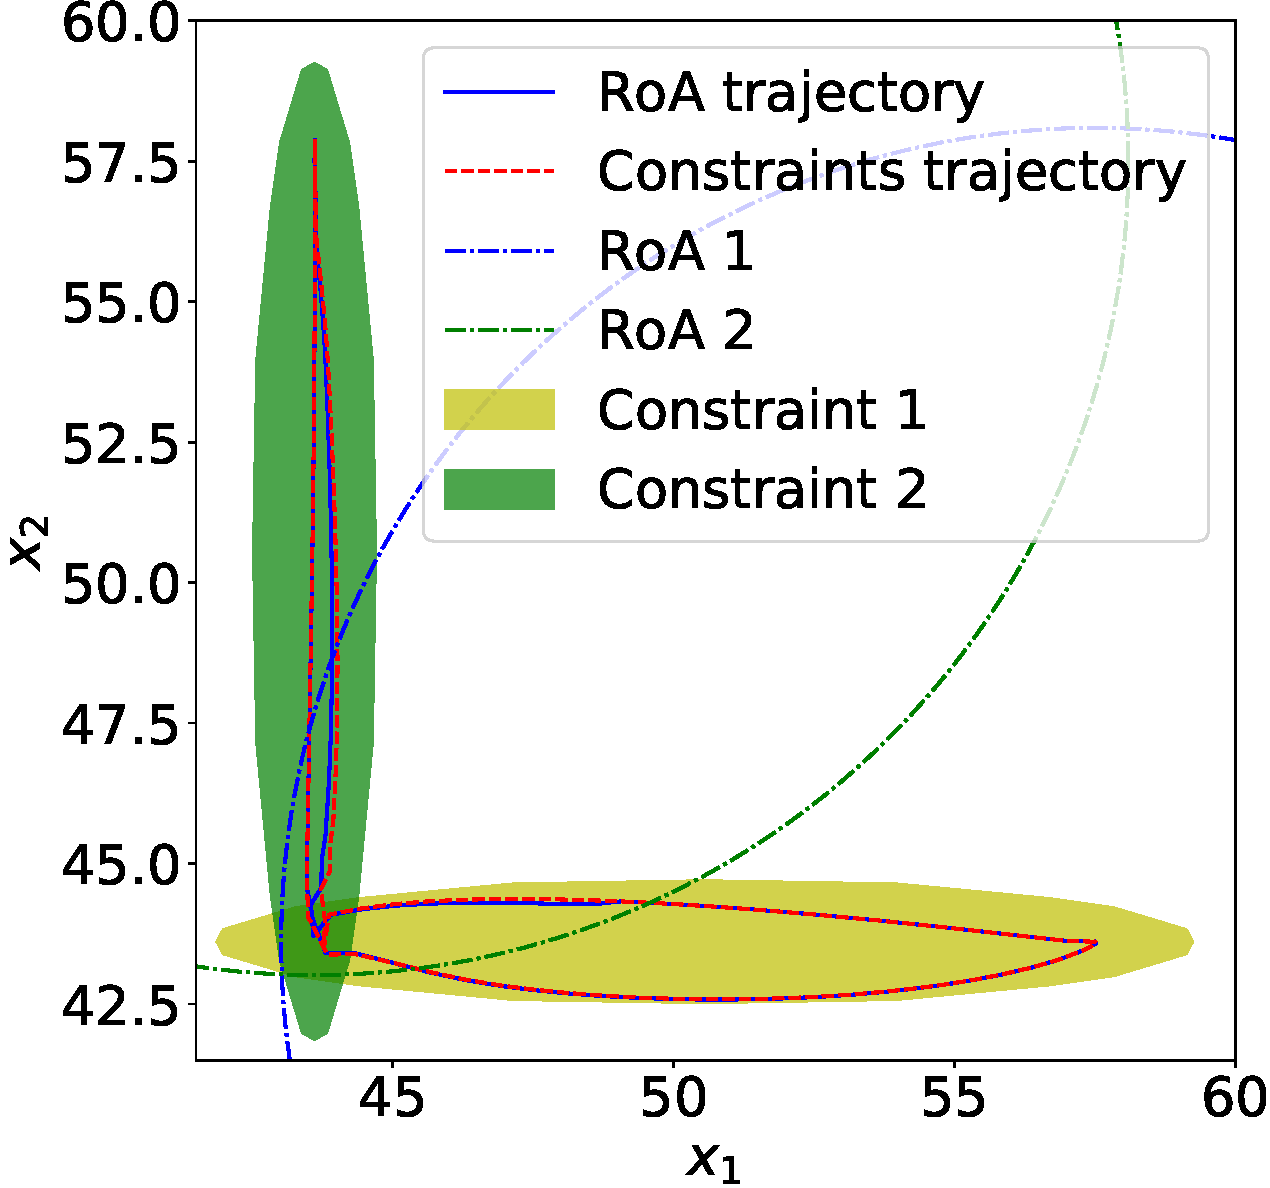
\includegraphics[height=0.75\textheight]{tanks-states}
    \caption{States trajectory for Example 1.}%
    \label{fig:level-system-control-states}
  \end{figure}
  \vspace*{\fill}
\end{slide}

\begin{slide}{System Description}
  \vspace*{\fill}
  \begin{figure}[ht!]
    \centering
    \captionsetup{justification=centering}
    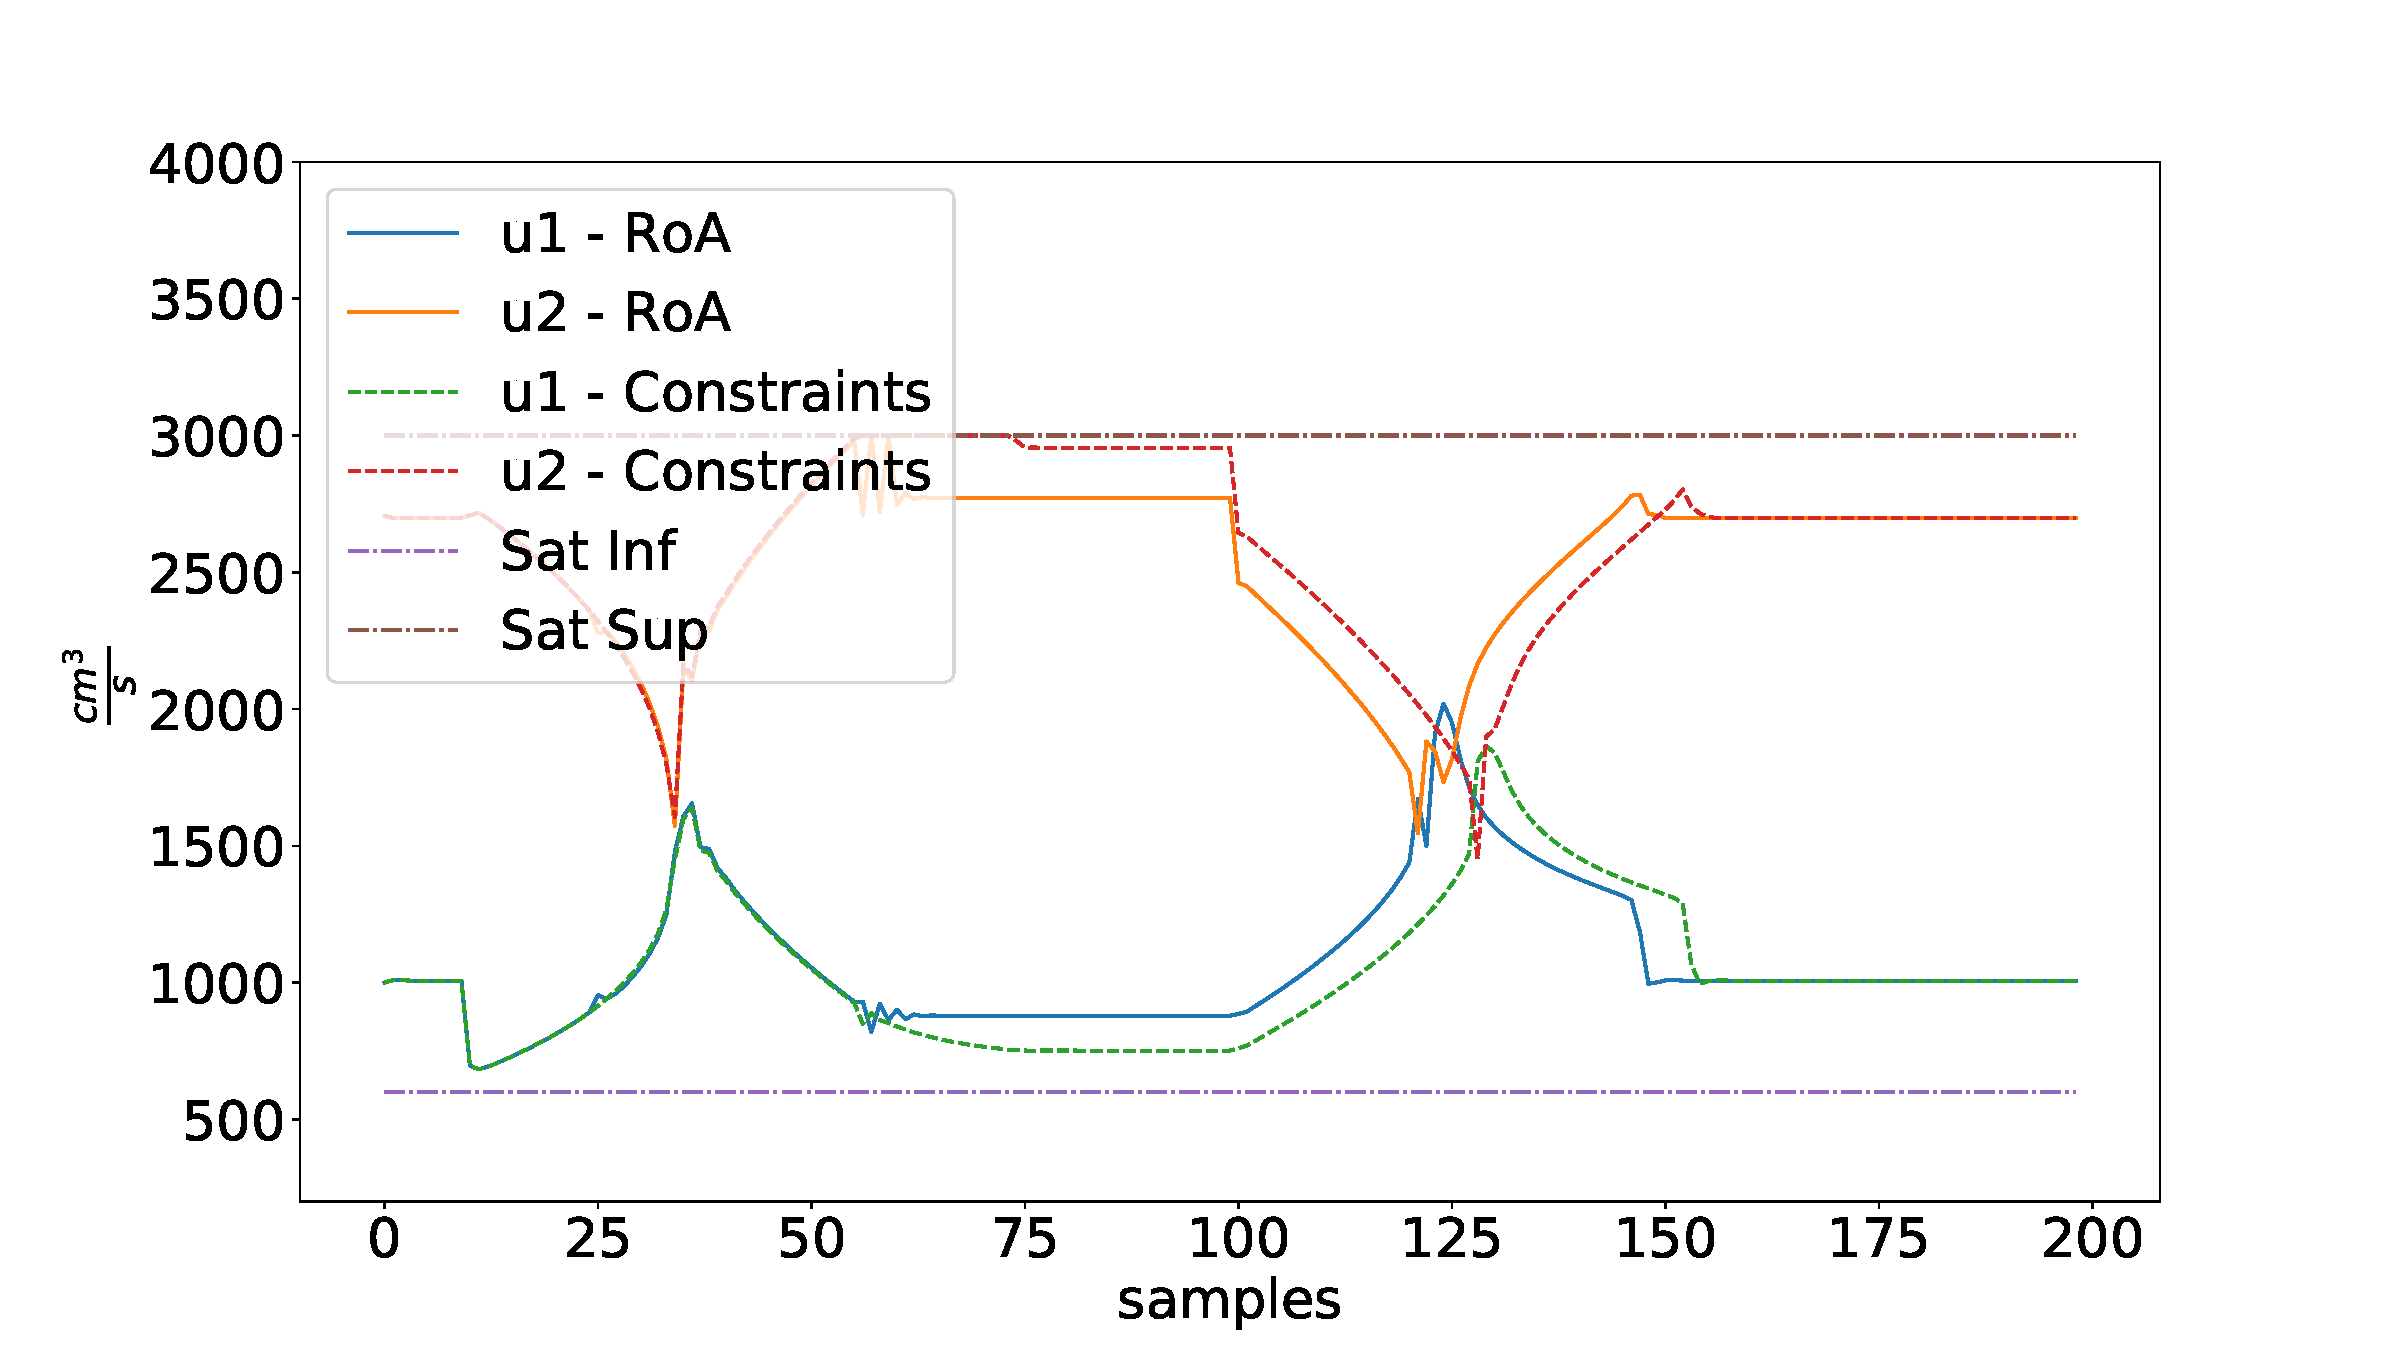
\includegraphics[height=0.75\textheight]{tanks-control-signal}
    \caption{Control signals for Example 1.}%
    \label{fig:level-system-control-signals}
  \end{figure}
\end{slide}

\subsection{Unstable System}%
\label{subsec:unstable-system}

\begin{slide}{Goal of Command Governor}
  \begin{columns}[c]
    \begin{column}{0.38\textwidth}
      \begin{equation}
        \begin{aligned}
          A_1 & =
          \begin{bmatrix}
            1 & 0.003 \\
            0 & 1
          \end{bmatrix}          \\
          A_2 & = \begin{bmatrix}
            1 & 0.0074 \\
            0 & 1.1
          \end{bmatrix}, \\
          B_1 & =
          \begin{bmatrix}
            0.0005 & 1.2\times{}10^{-6} \\
            0      & 0.0008
          \end{bmatrix},         \\
          B_2 & = \begin{bmatrix}
            0.0019 & 3.6\times{}10^{-5} \\
            0      & 0.011
          \end{bmatrix}, \\
          %
          C_1 & = C_2 =
          \begin{bmatrix}
            1 & 0 \\
            0 & 1
          \end{bmatrix}.         \\
        \end{aligned}
      \end{equation}
    \end{column}%
    \hfill%
    \begin{column}{0.58\textwidth}
      \begin{equation}
        \begin{aligned}
          x_{eq}^1 = \begin{bmatrix}
            1 \\ 1
          \end{bmatrix},
          u_{eq}^1 = \begin{bmatrix}
            -2 \\ \frac{-5}{4}
          \end{bmatrix},
          x_{eq}^2 = \begin{bmatrix}
            -1 \\ 1
          \end{bmatrix},
          u_{eq}^2 = \begin{bmatrix}
            \frac{-30}{19} \\ -10
          \end{bmatrix}.
        \end{aligned}
      \end{equation}
      \begin{equation}
        \resizebox{0.8\linewidth}{!}{%
          \(\begin{aligned}
            K_1 & = \begin{bmatrix}
              -2.669\times{}10^3   & -1.993             & -6.741\times{}10^2    & 1.010              \\
              3.582\times{}10^{-4} & -1.669\times{}10^3 & -3.103\times{}10^{-4} & -4.210\times{}10^2
            \end{bmatrix}, \\
            K_2 & = \begin{bmatrix}
              -7.034\times{}10^2    & -1.268             & -1.769\times{}10^2    & 6.097\times{}10^{-1} \\
              -3.903\times{}10^{-6} & -1.370\times{}10^2 & -1.292\times{}10^{-5} & -3.202\times{}10^1
            \end{bmatrix}.
          \end{aligned}\)
        }
      \end{equation}
    \end{column}%
  \end{columns}
\end{slide}

\begin{slide}{Goal of Command Governor}
  \begin{figure}[ht!]
    \centering
    \captionsetup{justification=centering}
    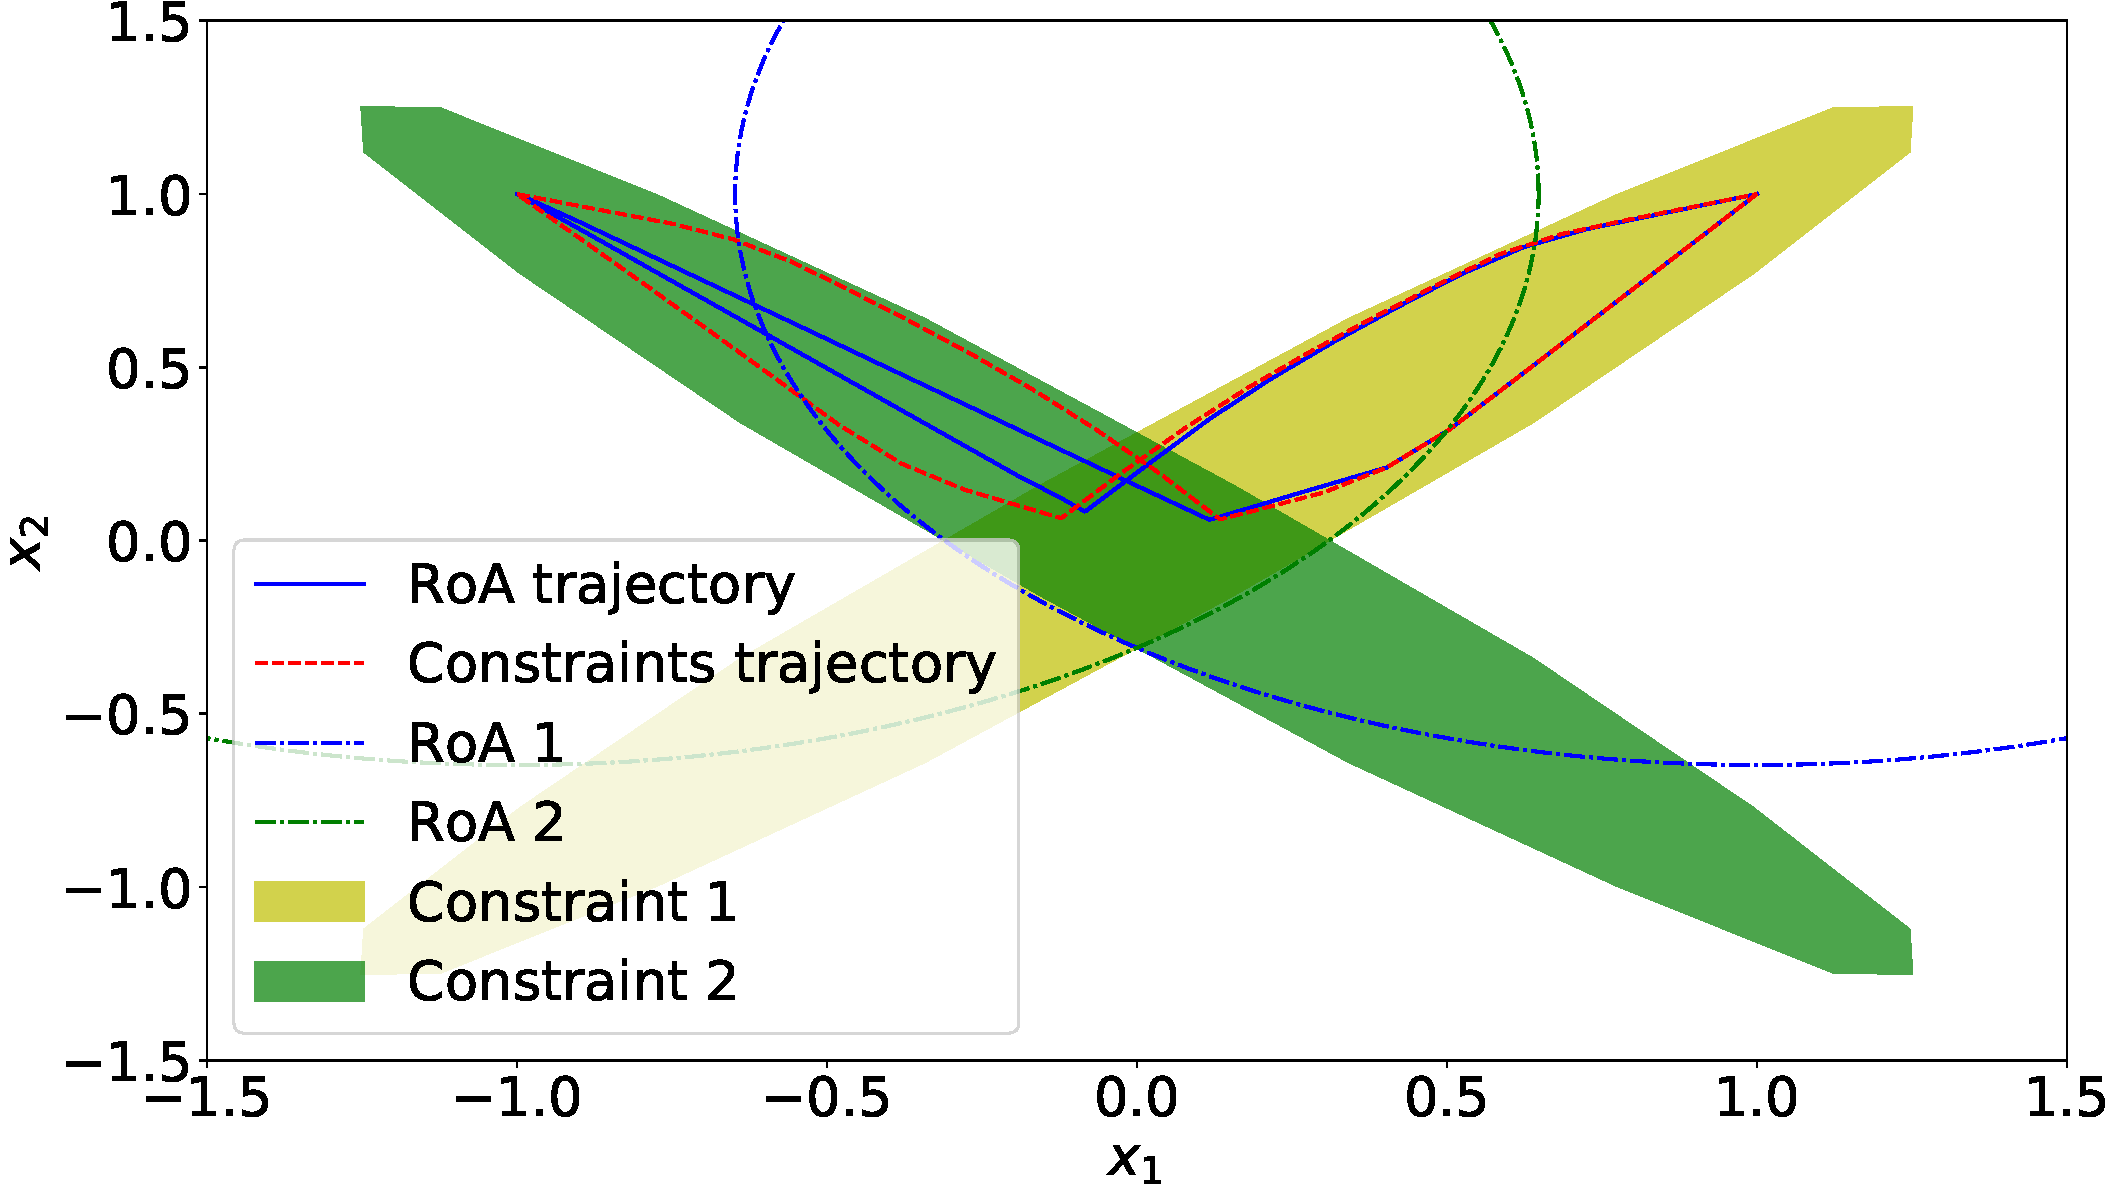
\includegraphics[height=0.75\textheight]{unstable_states}
    \caption{States trajectory for Example 2}%
    \label{fig:unstable-states}
  \end{figure}
\end{slide}

\begin{slide}{Goal of Command Governor}
  \begin{figure}[ht!]
    \centering
    \captionsetup{justification=centering}
    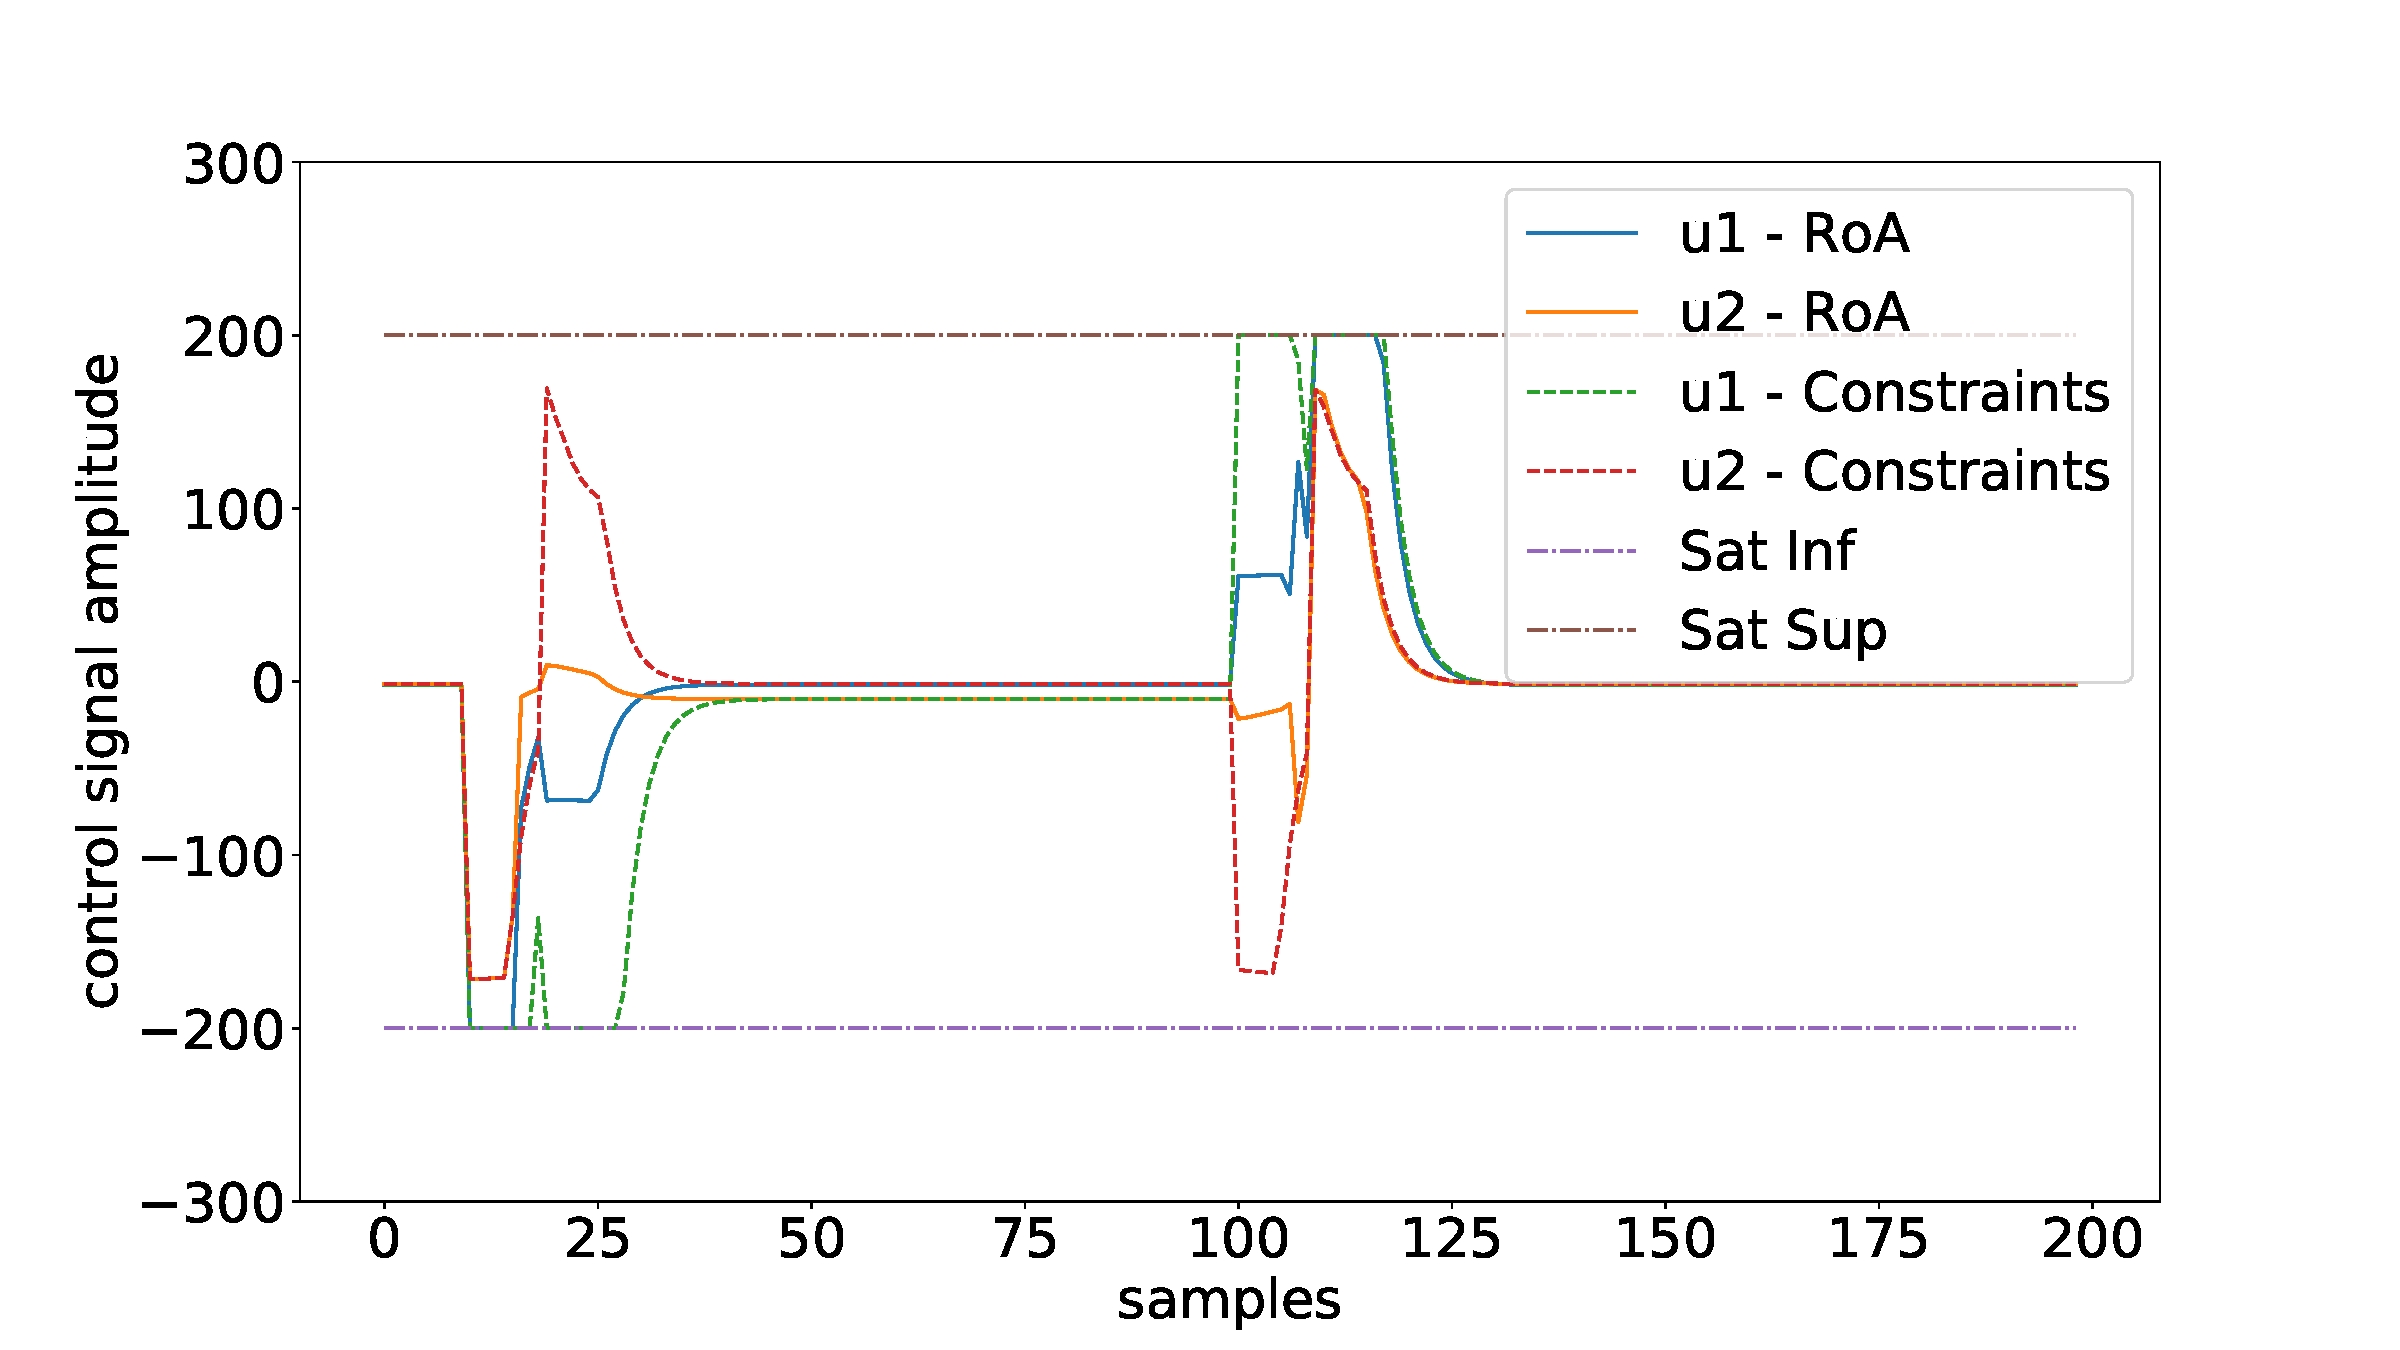
\includegraphics[height=0.75\textheight]{unstable_control_signal}
    \caption{Control signals for Example 2}%
    \label{fig:unstable-control-signals}
  \end{figure}
\end{slide}

\subsection{Cessna 182}%
\label{subsec:cessna}

\begin{slide}{Goal of Command Governor}
  \begin{figure}[ht!]
    \centering \captionsetup{justification=centering}
    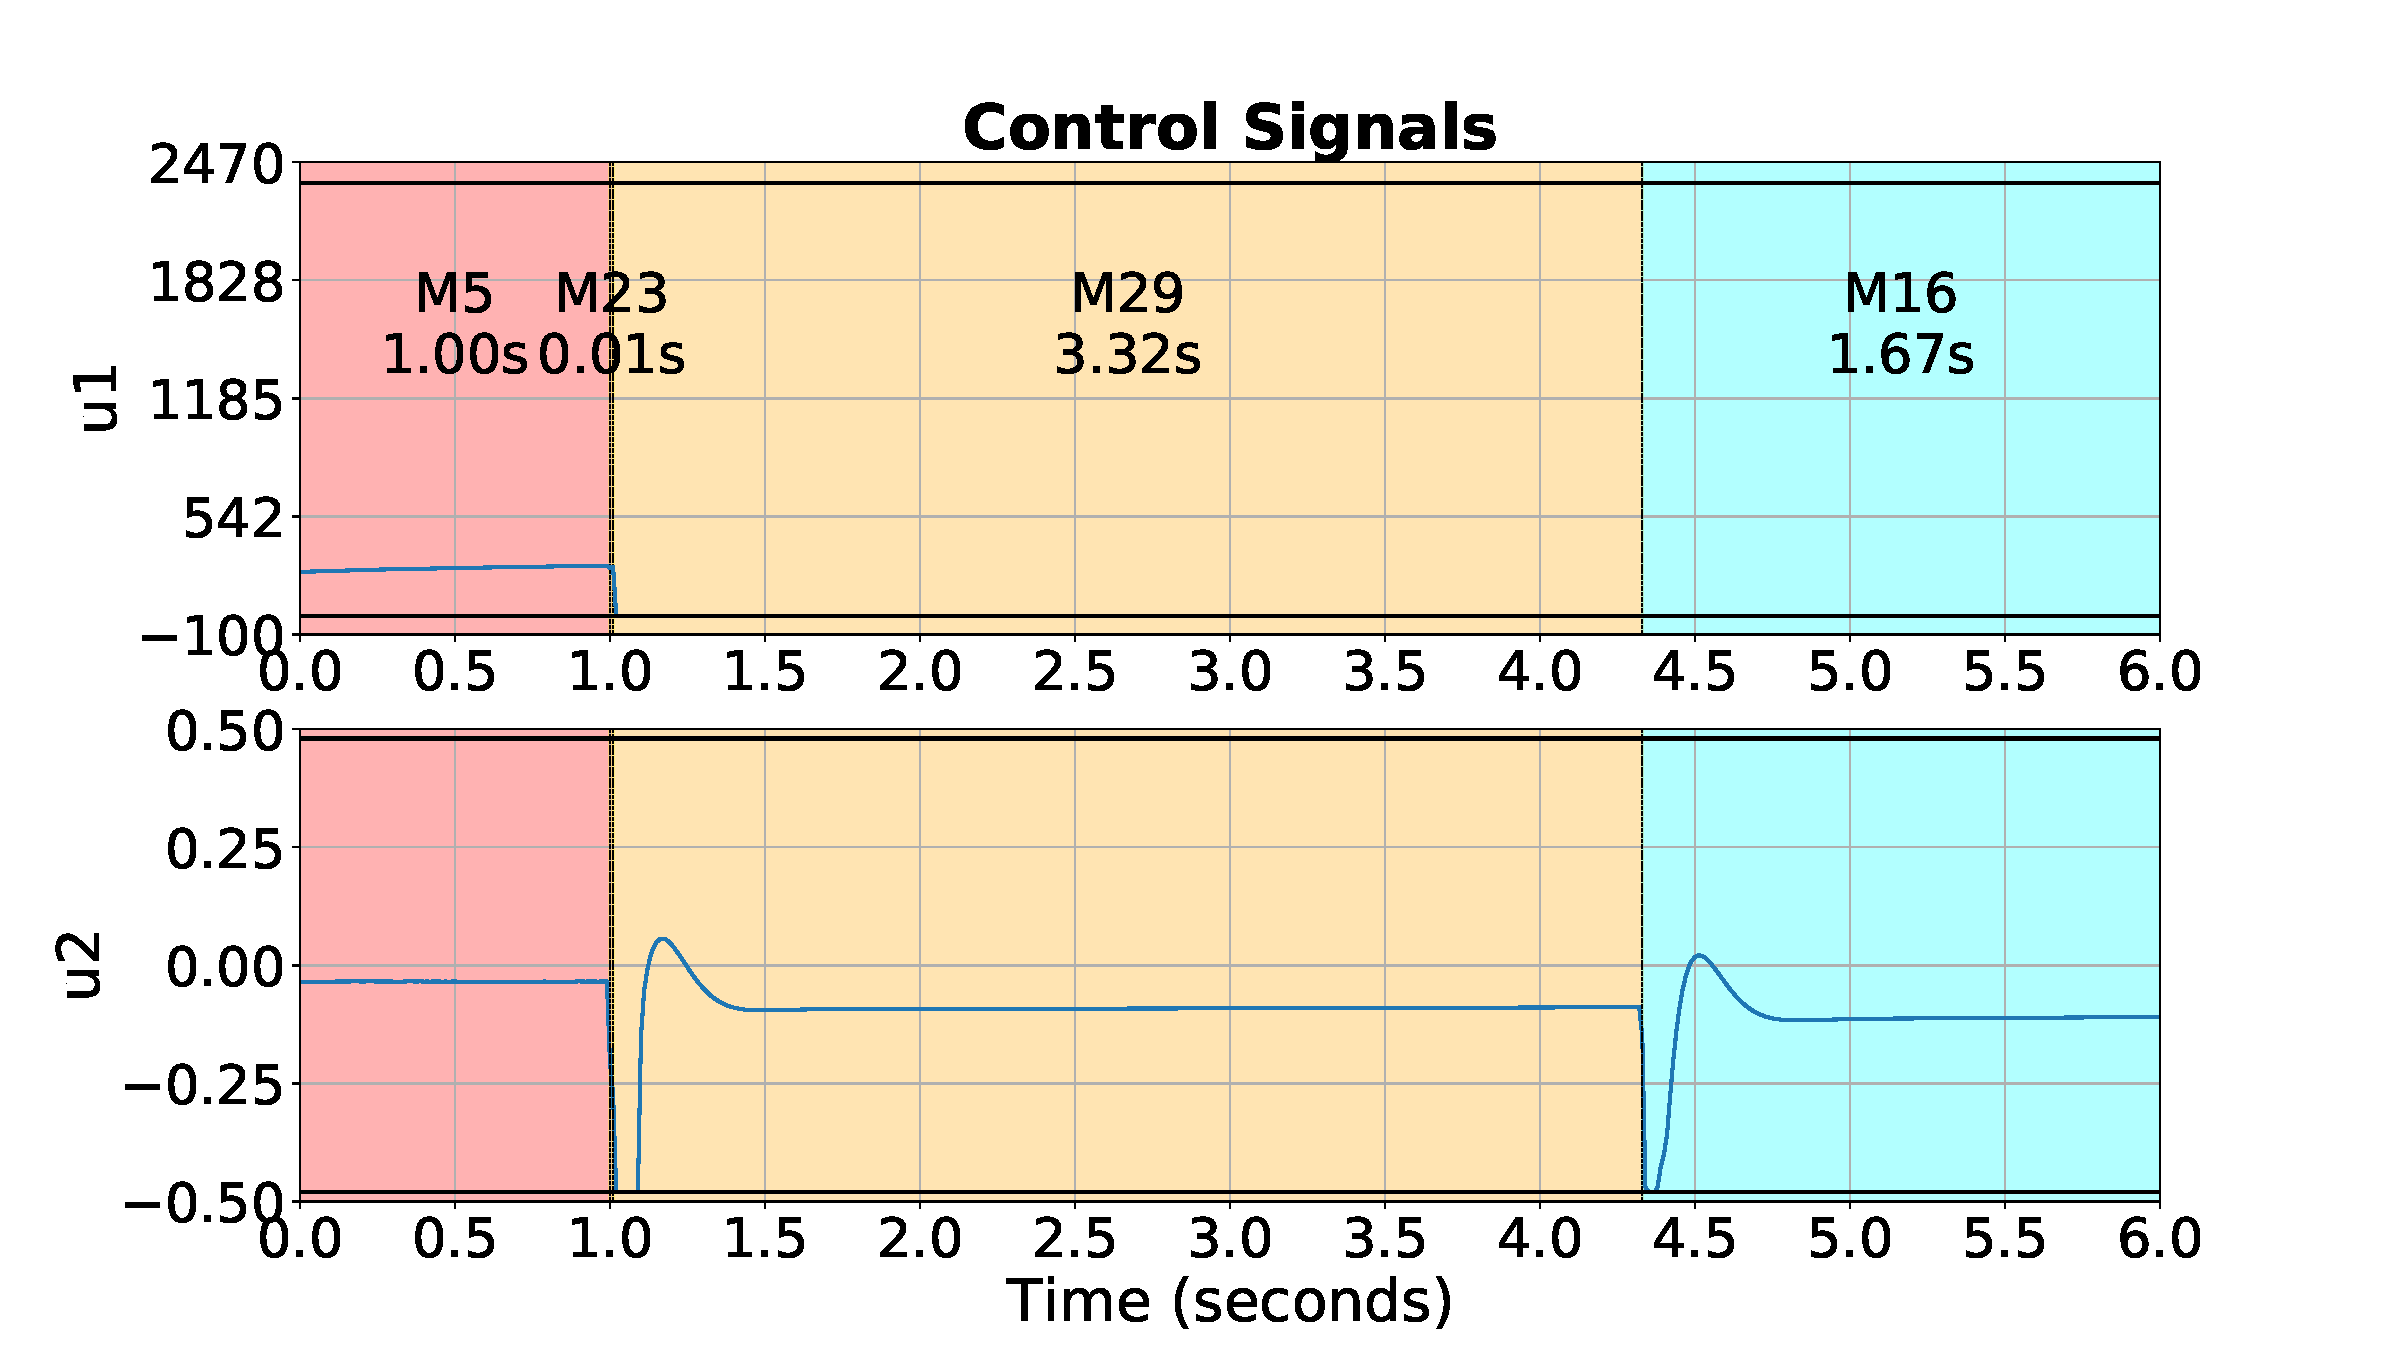
\includegraphics[height=0.75\textheight]{cessna-u}
    \caption{Cessna simulation control signal}%
    \label{fig:cessna-u}
  \end{figure}
\end{slide}

\begin{slide}{Goal of Command Governor}
  \begin{figure}[ht!]
    \centering \captionsetup{justification=centering}
    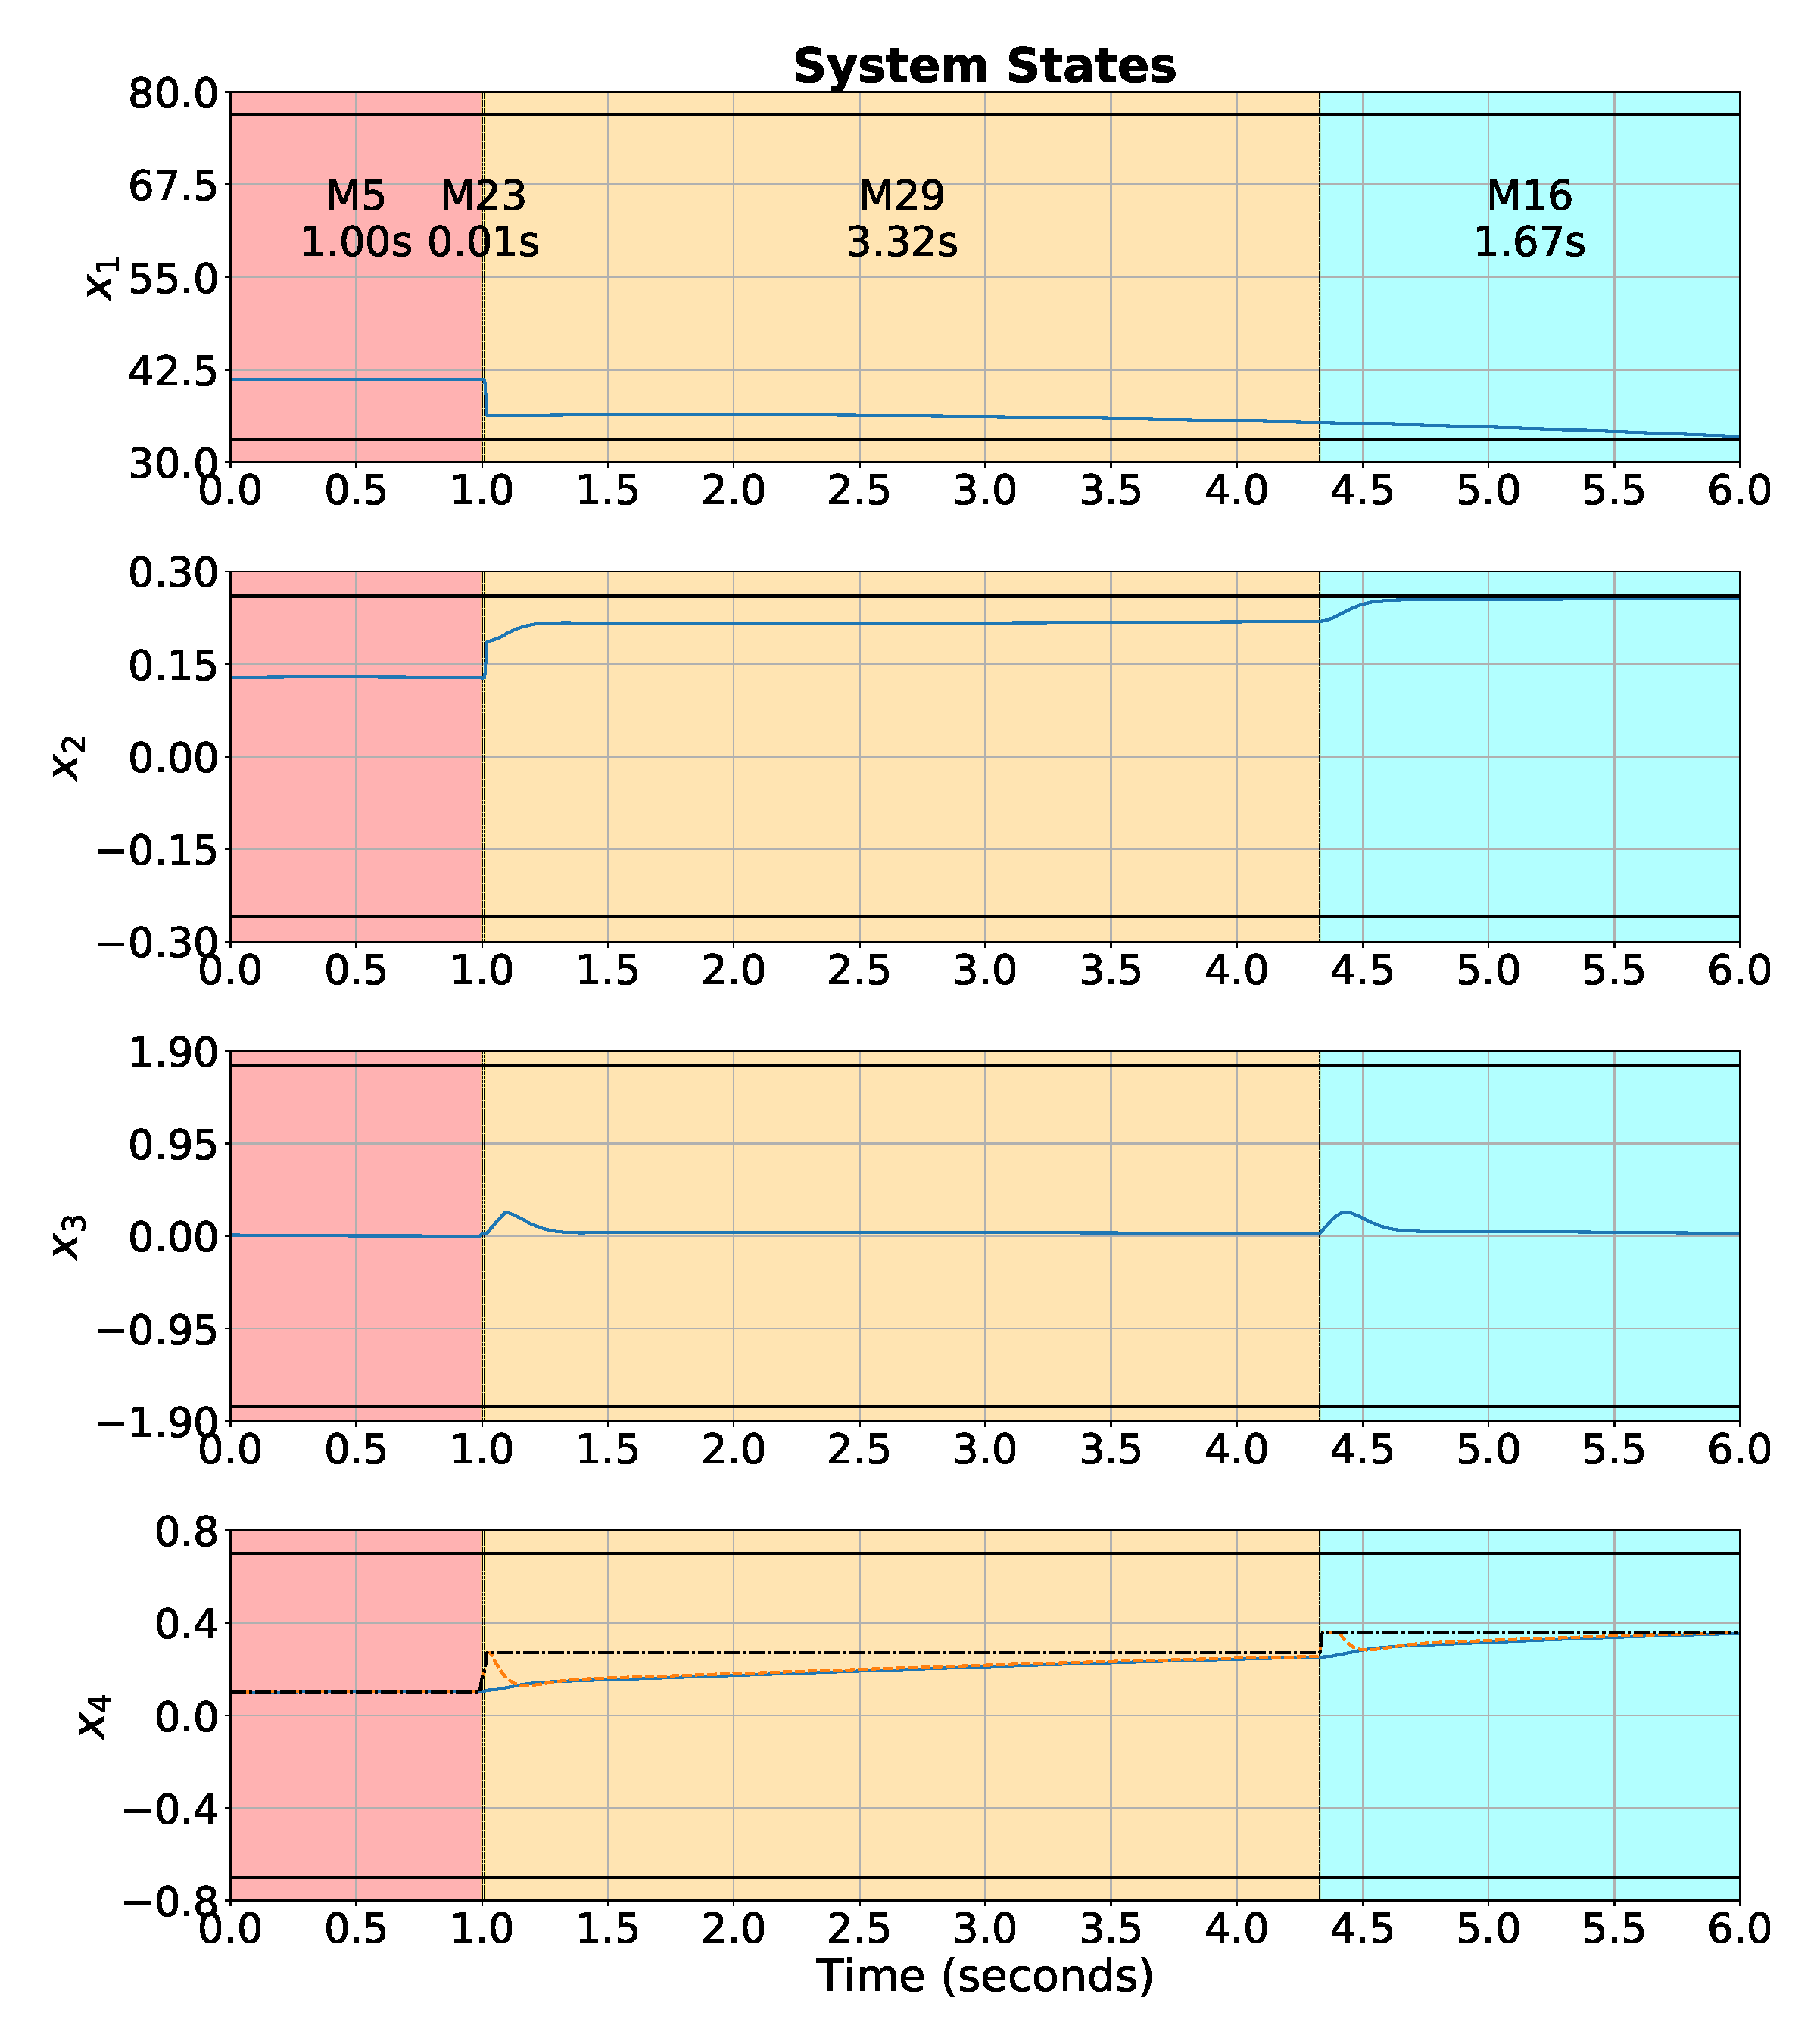
\includegraphics[height=0.75\textheight]{cessna-x}
    \caption{Cessna simulation states}%
    \label{fig:cessna-x}
  \end{figure}
\end{slide}

\subsection{Coupled Tanks}%
\label{subsec:tanks}

\begin{slide}{Goal of Command Governor}
  \begin{figure}[ht!]
    \centering \captionsetup{justification=centering}
    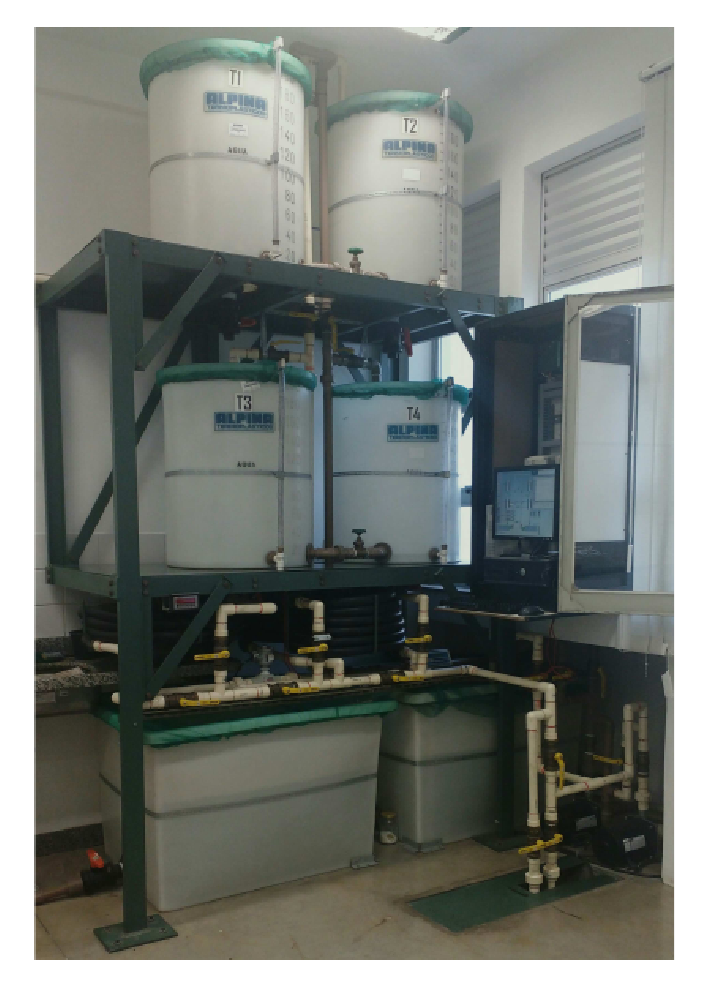
\includegraphics[height=.75\textheight]{tanks-real}
    \caption{Tank system}%
    \label{fig:tanks-real}
  \end{figure}
\end{slide}

\begin{slide}{Goal of Command Governor}
  \begin{figure}[ht!]
    \centering \captionsetup{justification=centering}
    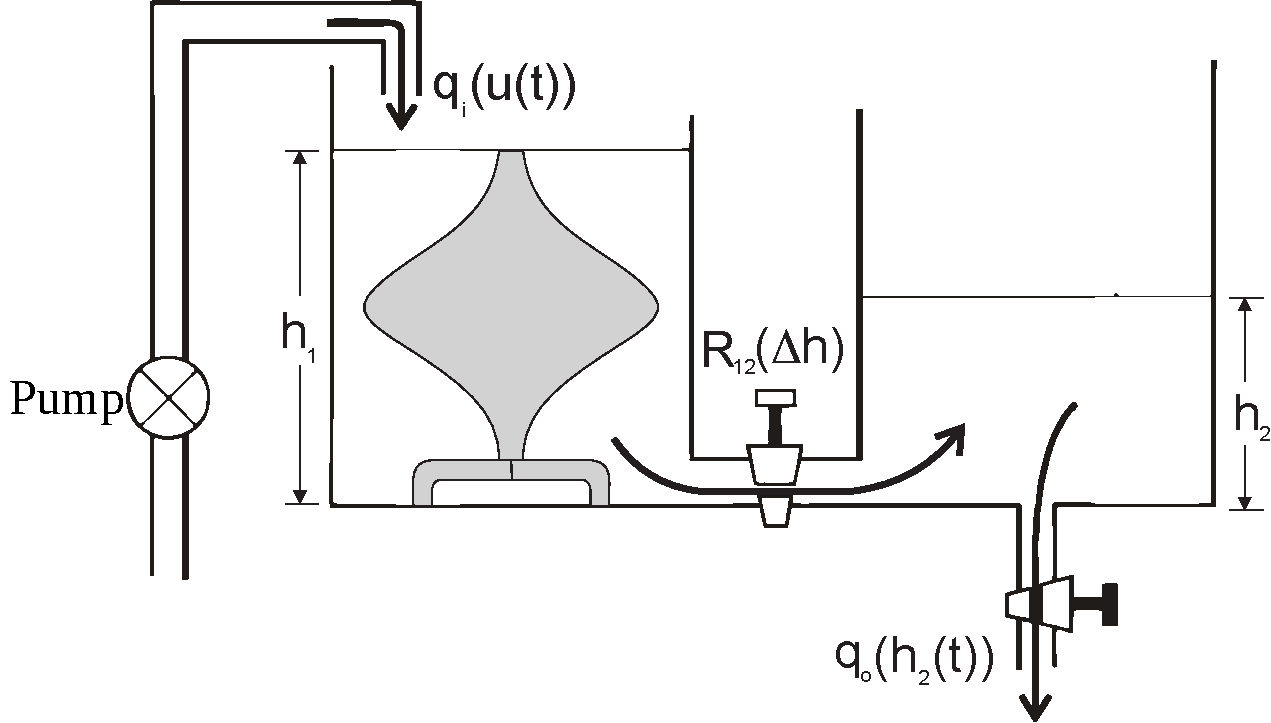
\includegraphics[height=.75\textheight]{tanks}
    \caption{Tank system diagram}%
    \label{fig:tanks}
  \end{figure}
\end{slide}

\begin{slide}{Goal of Command Governor}
  \begin{equation}
    \label{eq:t1-area}
    A_{1}(h_{1}(t)) = \frac{3r}{5} \left(
    2.7r - \frac{\cos(2.5\pi{}((h_{1}(t)-8)\times{}10^{-2}-\mu))}{\sigma{}\sqrt{2\pi}}
    e^{-\frac{((h_{1}(t)-8)\times{}10^{-2}-\mu^{2})^{2}}{2\sigma^{2}}}
    \right)
  \end{equation}
\end{slide}

\begin{slide}{Goal of Command Governor}
  \begin{equation}
    \label{eq:formula-height-variation}
    \begin{aligned}
      \dot{h}_1(t) & = \frac{R_{12}(h_{1}(t),h_{2}(t))\times{}K_{b}\times{}u(t)-h_{1}(t)+h_{2}(t)}
      {A_{1}(h_{1}(t))\times{}R_{12}(h_{1}(t),h_{2}(t))},                                                                \\
      \dot{h}_2(t) & = \frac{h_{1}(t)-h_{2}(t)}{R_{12}(h_{1}(t),h_{2}(t))\times{}A_{2}} - \frac{q_{o}(h_{2}(t))}{A_{2}}.
    \end{aligned}
  \end{equation}
\end{slide}

\begin{slide}{Goal of Command Governor}
  \begin{equation}
    \begin{aligned}
      \label{eq:op-points}
      \left[\begin{array}{c|c}
          x_{eq}^{\top} & u_{eq} \\
          \hline
          A             & B
        \end{array}\right]_{1} & = \left[\begin{array}{cc|c}
          19.5  & 5    & 15     \\
          \hline
          0.91  & 0.14 & 0.028  \\
          0.085 & 0.9  & 0.0013
        \end{array}\right], \\
      \left[\begin{array}{c|c}
          x_{eq}^{\top} & u_{eq} \\
          \hline
          A             & B
        \end{array}\right]_{2} & = \left[\begin{array}{cc|c}
          27.5  & 11.6 & 20     \\
          \hline
          0.94  & 0.19 & 0.04   \\
          0.084 & 0.9  & 0.0018
        \end{array}\right], \\
      \left[\begin{array}{c|c}
          x_{eq}^{\top} & u_{eq} \\
          \hline
          A             & B
        \end{array}\right]_{3} & = \left[\begin{array}{cc|c}
          37.3  & 17.8 & 25     \\
          \hline
          1.1   & 0.47 & 0.1    \\
          0.086 & 0.92 & 0.0042
        \end{array}\right], \\
      \left[\begin{array}{c|c}
          x_{eq}^{\top} & u_{eq} \\
          \hline
          A             & B
        \end{array}\right]_{4} & = \left[\begin{array}{cc|c}
          47.4  & 24.9 & 30     \\
          \hline
          0.49  & 0.96 & 0.22   \\
          0.053 & 0.95 & 0.0096
        \end{array}\right].
    \end{aligned}
  \end{equation}
\end{slide}

\begin{slide}{Goal of Command Governor}
  \begin{equation}
    \begin{aligned}
      K_{1} & = \begin{bmatrix} -12.884 & -97.540 & -13.975 \end{bmatrix}, \\
      K_{2} & = \begin{bmatrix} -10.054 & -73.777 & -10.523 \end{bmatrix}, \\
      K_{3} & = \begin{bmatrix} -5.840  & -31.622 & -4.148 \end{bmatrix}, \\
      K_{4} & = \begin{bmatrix} -1.832  & -21.527 & -4.177 \end{bmatrix}.
    \end{aligned}
  \end{equation}
\end{slide}

\begin{slide}{Goal of Command Governor}
  \begin{figure}[ht!]
    \centering \captionsetup{justification=centering}
    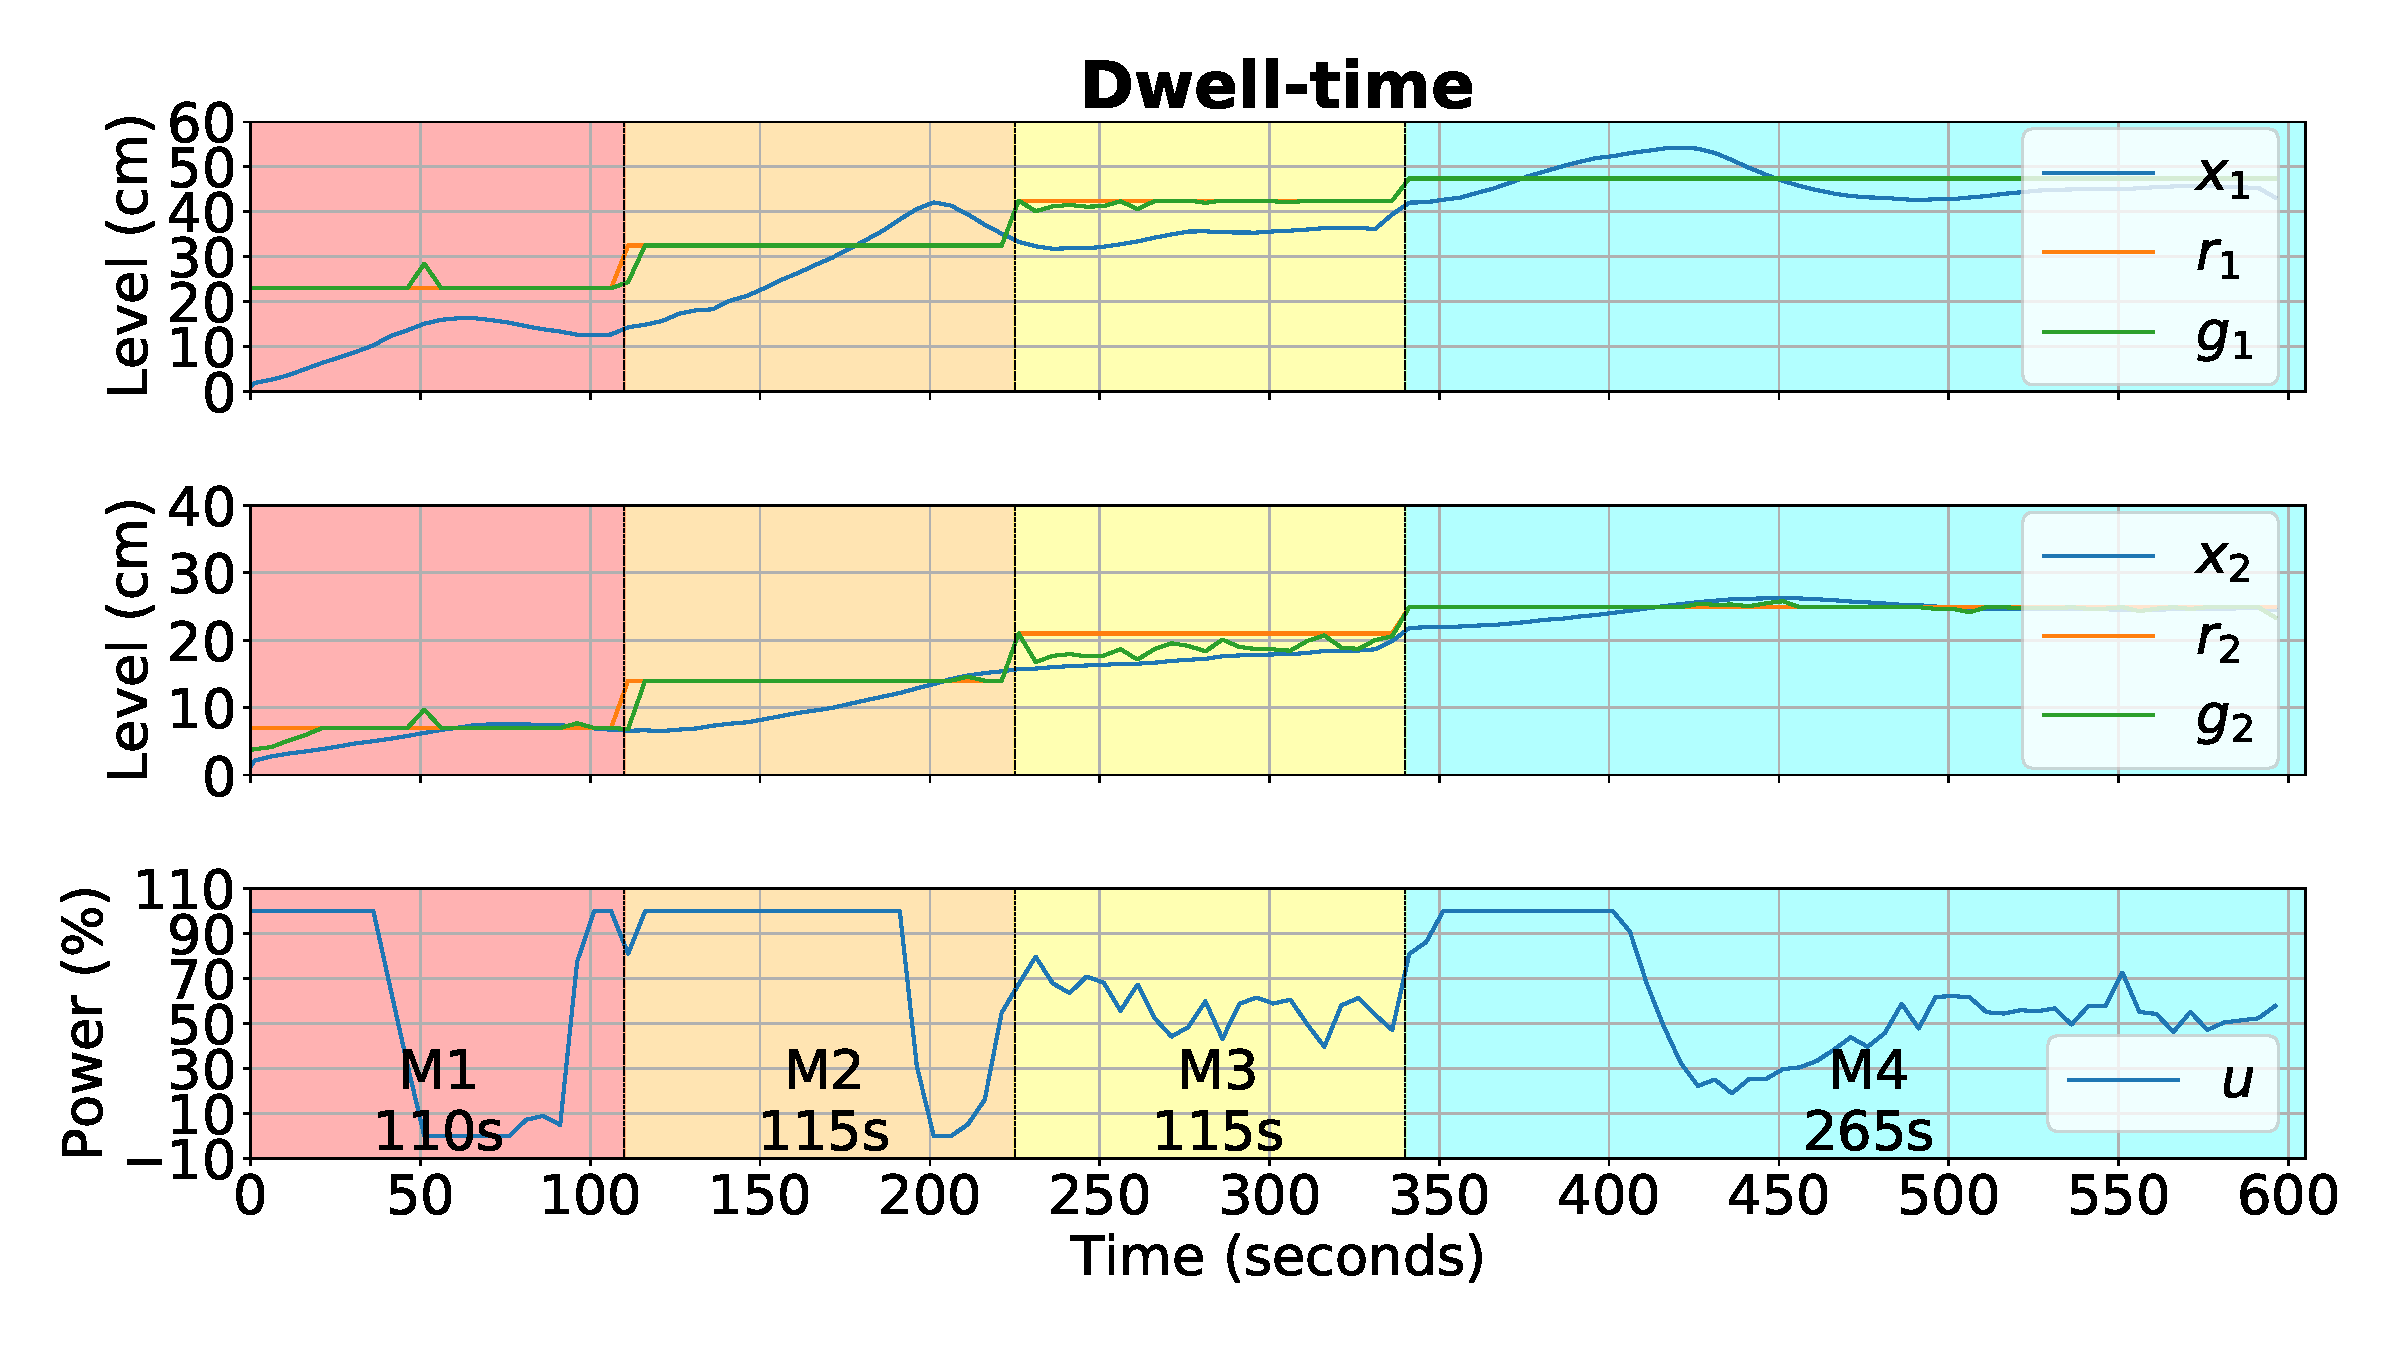
\includegraphics[width=0.7\linewidth]{tanks-dwell}
    \caption{Dwell-time approach}%
    \label{fig:tanks-dwell}
  \end{figure}
\end{slide}

\begin{slide}{Goal of Command Governor}
  \begin{figure}[ht!]
    \centering \captionsetup{justification=centering}
    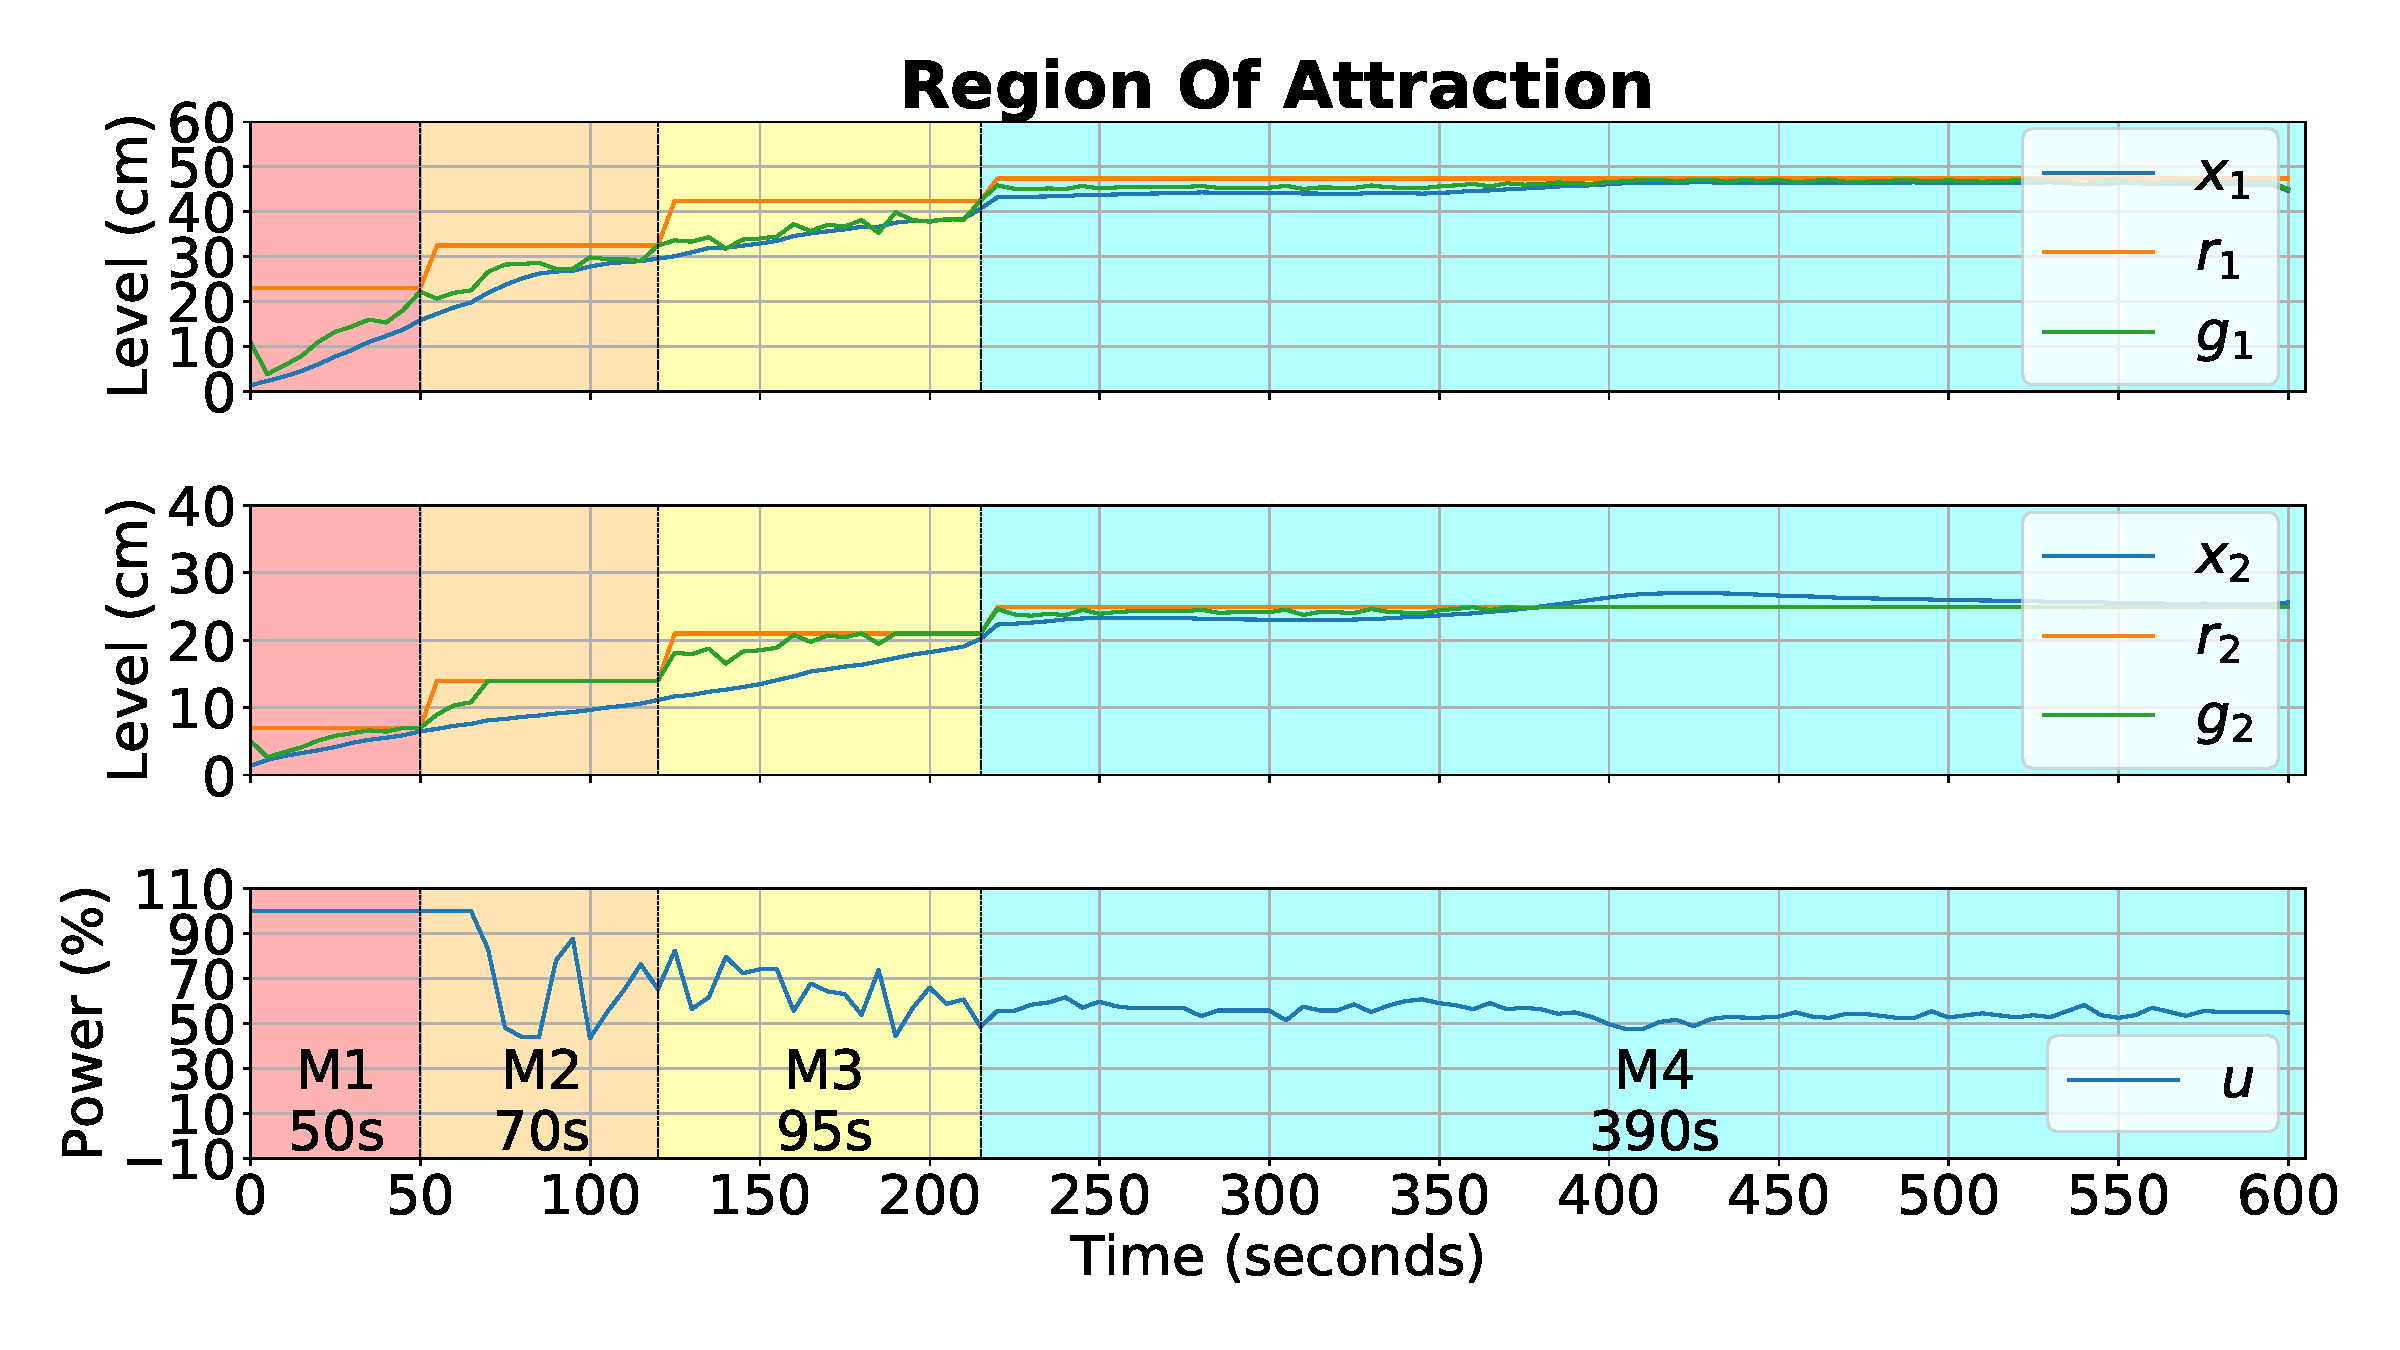
\includegraphics[width=0.7\linewidth]{tanks-roa}
    \caption{Proposed RoA-based approach}%
    \label{fig:tanks-roa}
  \end{figure}
\end{slide}

% !TeX root = document.tex
% !TeX encoding = UTF-8 Unicode

\subsection{Results}%
\label{subsec:ts-results}

\begin{slide}{Observer}
  \begin{columns}[c]
    \begin{column}{0.55\textwidth}
      \begin{align}
        \mathcal{A}    & = \begin{bmatrix}
                             -1 & 1  & 0     & 0  & 0  \\
                             -1 & -1 & 1.495 & 0  & 0  \\
                             0  & 0  & -2    & 1  & 0  \\
                             0  & 0  & 0     & -3 & 1  \\
                             0  & 0  & 0     & 0  & -5
                           \end{bmatrix},        \\
        \mathcal{B}    & =\begin{bmatrix}
                            0 \\ 0 \\ 0 \\ 0 \\ 16
                          \end{bmatrix},
        \mathcal{C} = \begin{bmatrix}
                        -5.517 \\ 2.759 \\ 0 \\ 0 \\ 0
                      \end{bmatrix}^{\top},
        \mathcal{D} = 0                                     \\
        \textrm{poles} & = \{-1\pm{}1\imath{}, -2, -3, -5\}
      \end{align}
    \end{column}%
    \hfill%
    \begin{column}{0.55\textwidth}
      \begin{figure}[ht!]
        \centering
        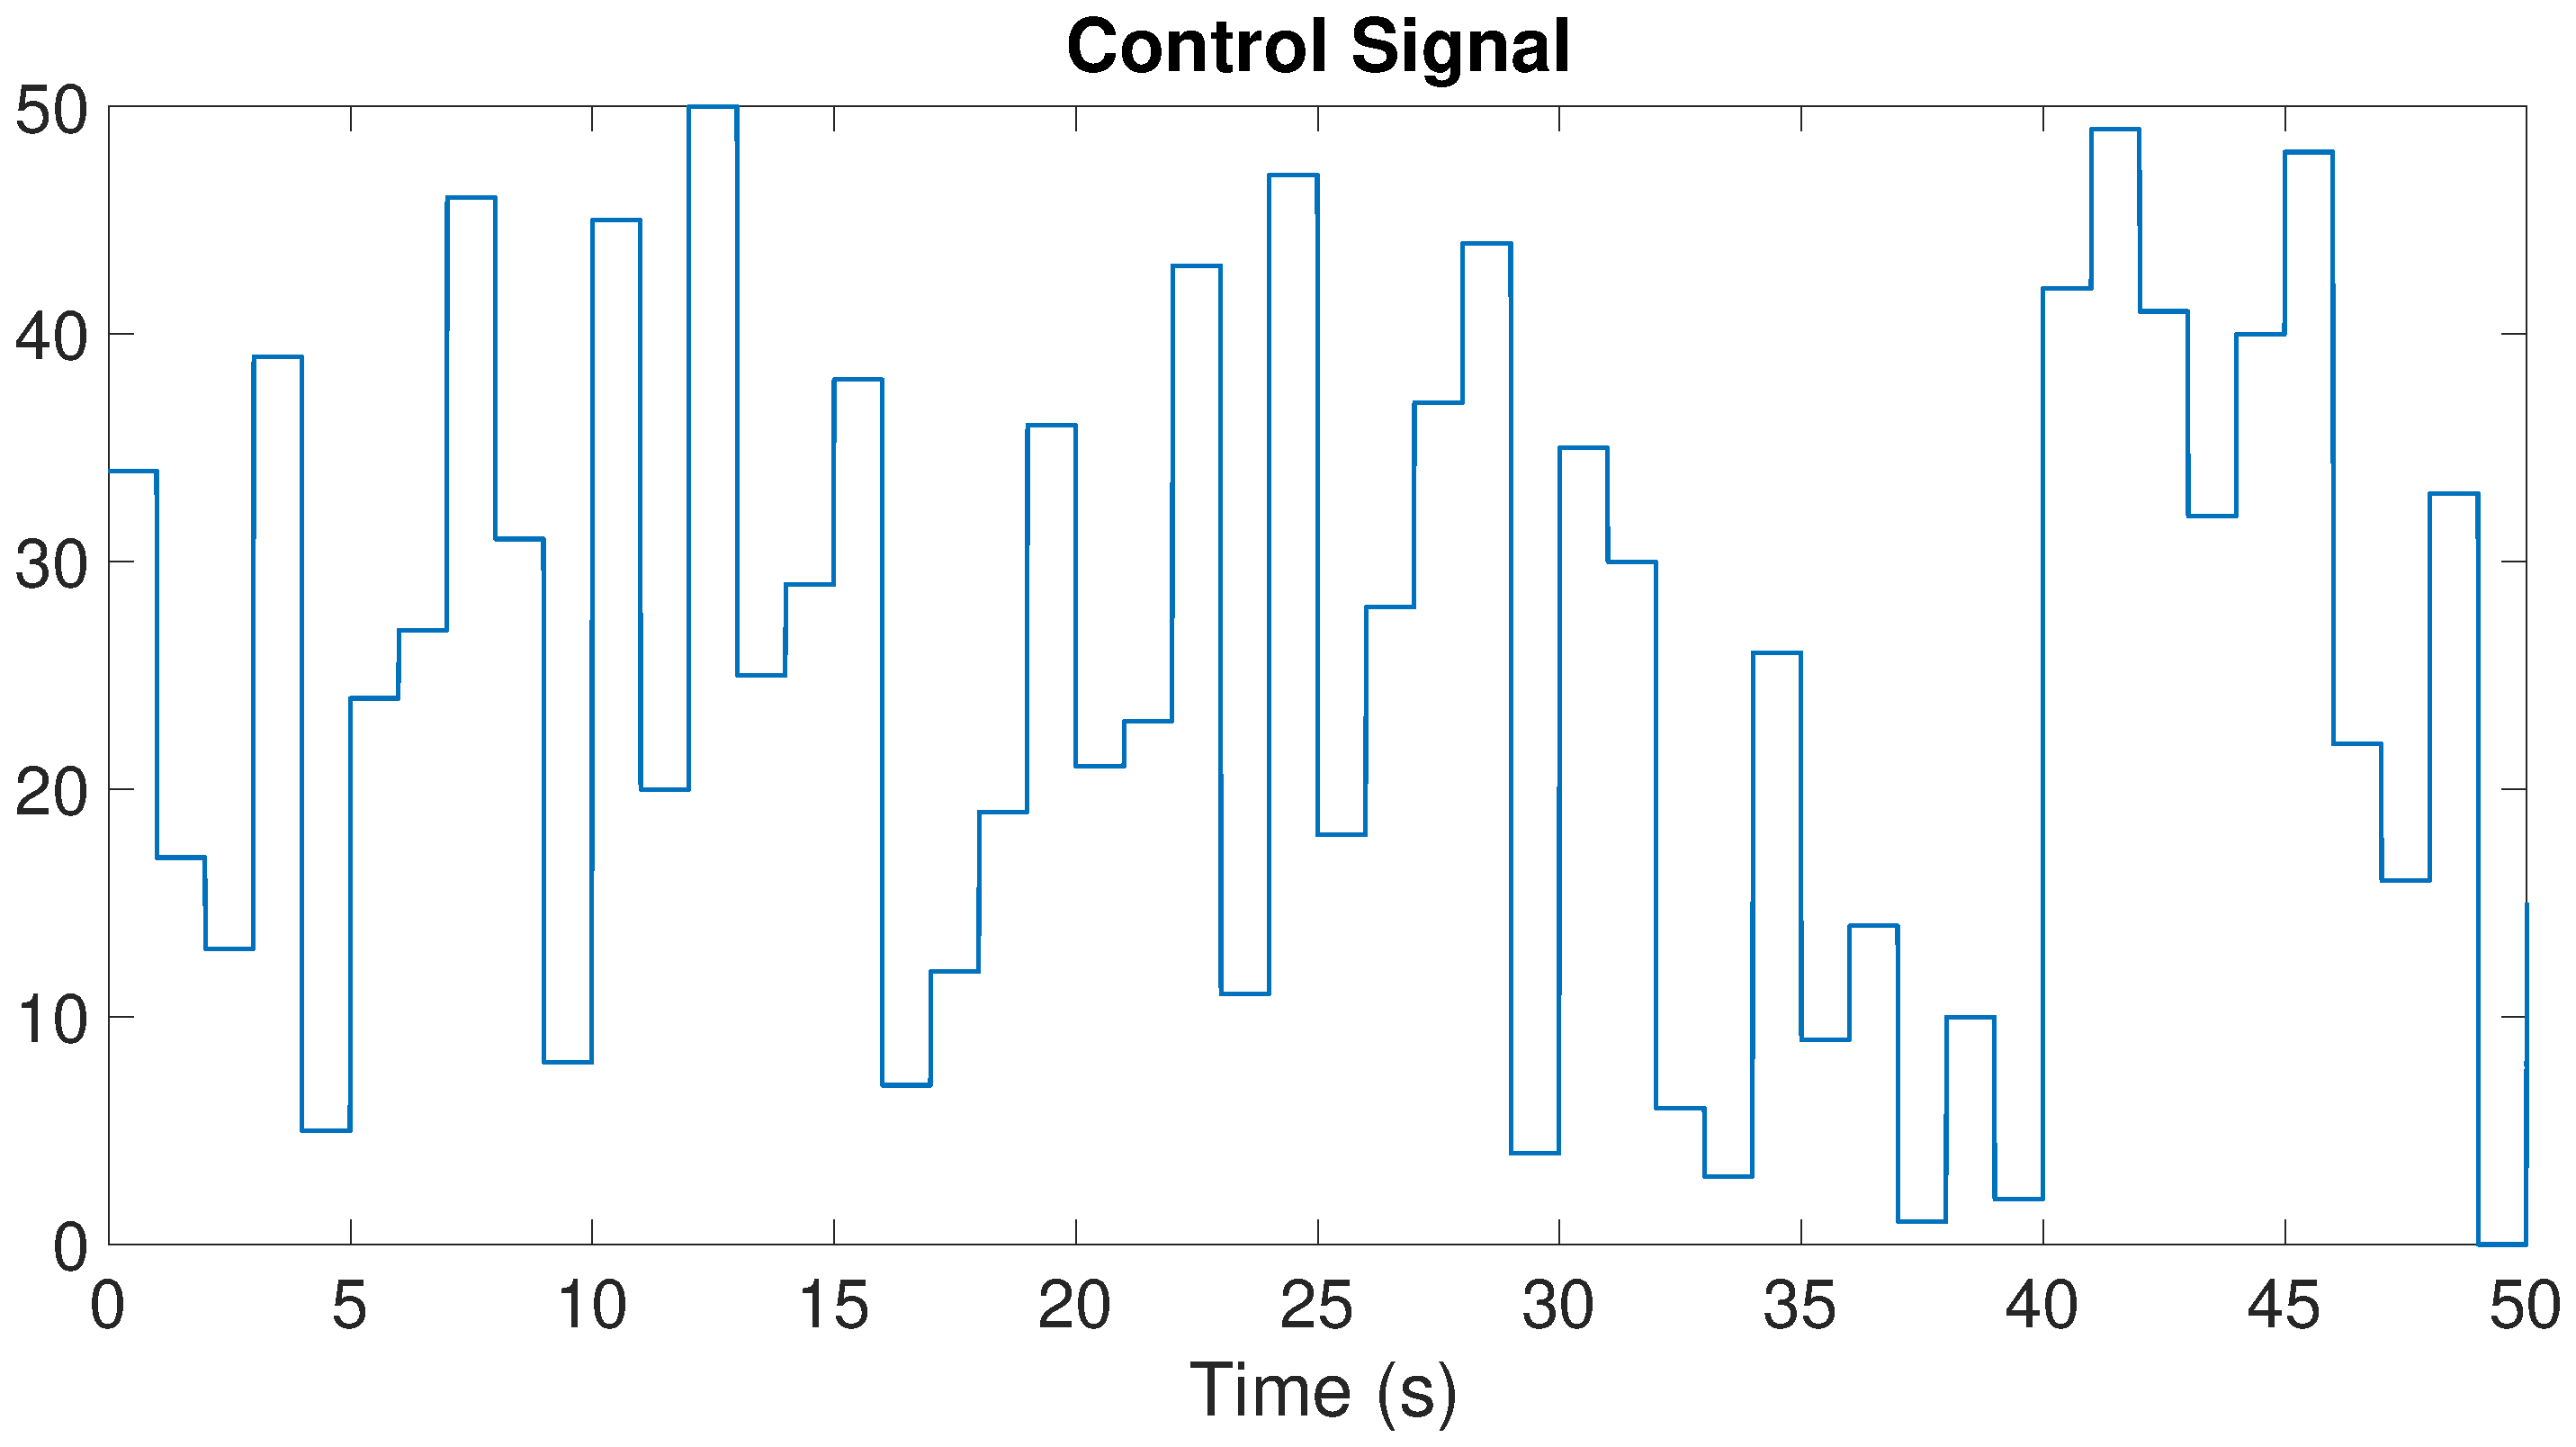
\includegraphics[width=\linewidth]{stair-input-u}
        \caption{Control Signal.}%
      \end{figure}
    \end{column}%
  \end{columns}
\end{slide}

\begin{slide}{Observer}
  \begin{columns}[c]
    \begin{column}{0.55\textwidth}
      \begin{figure}[ht!]
        \centering
        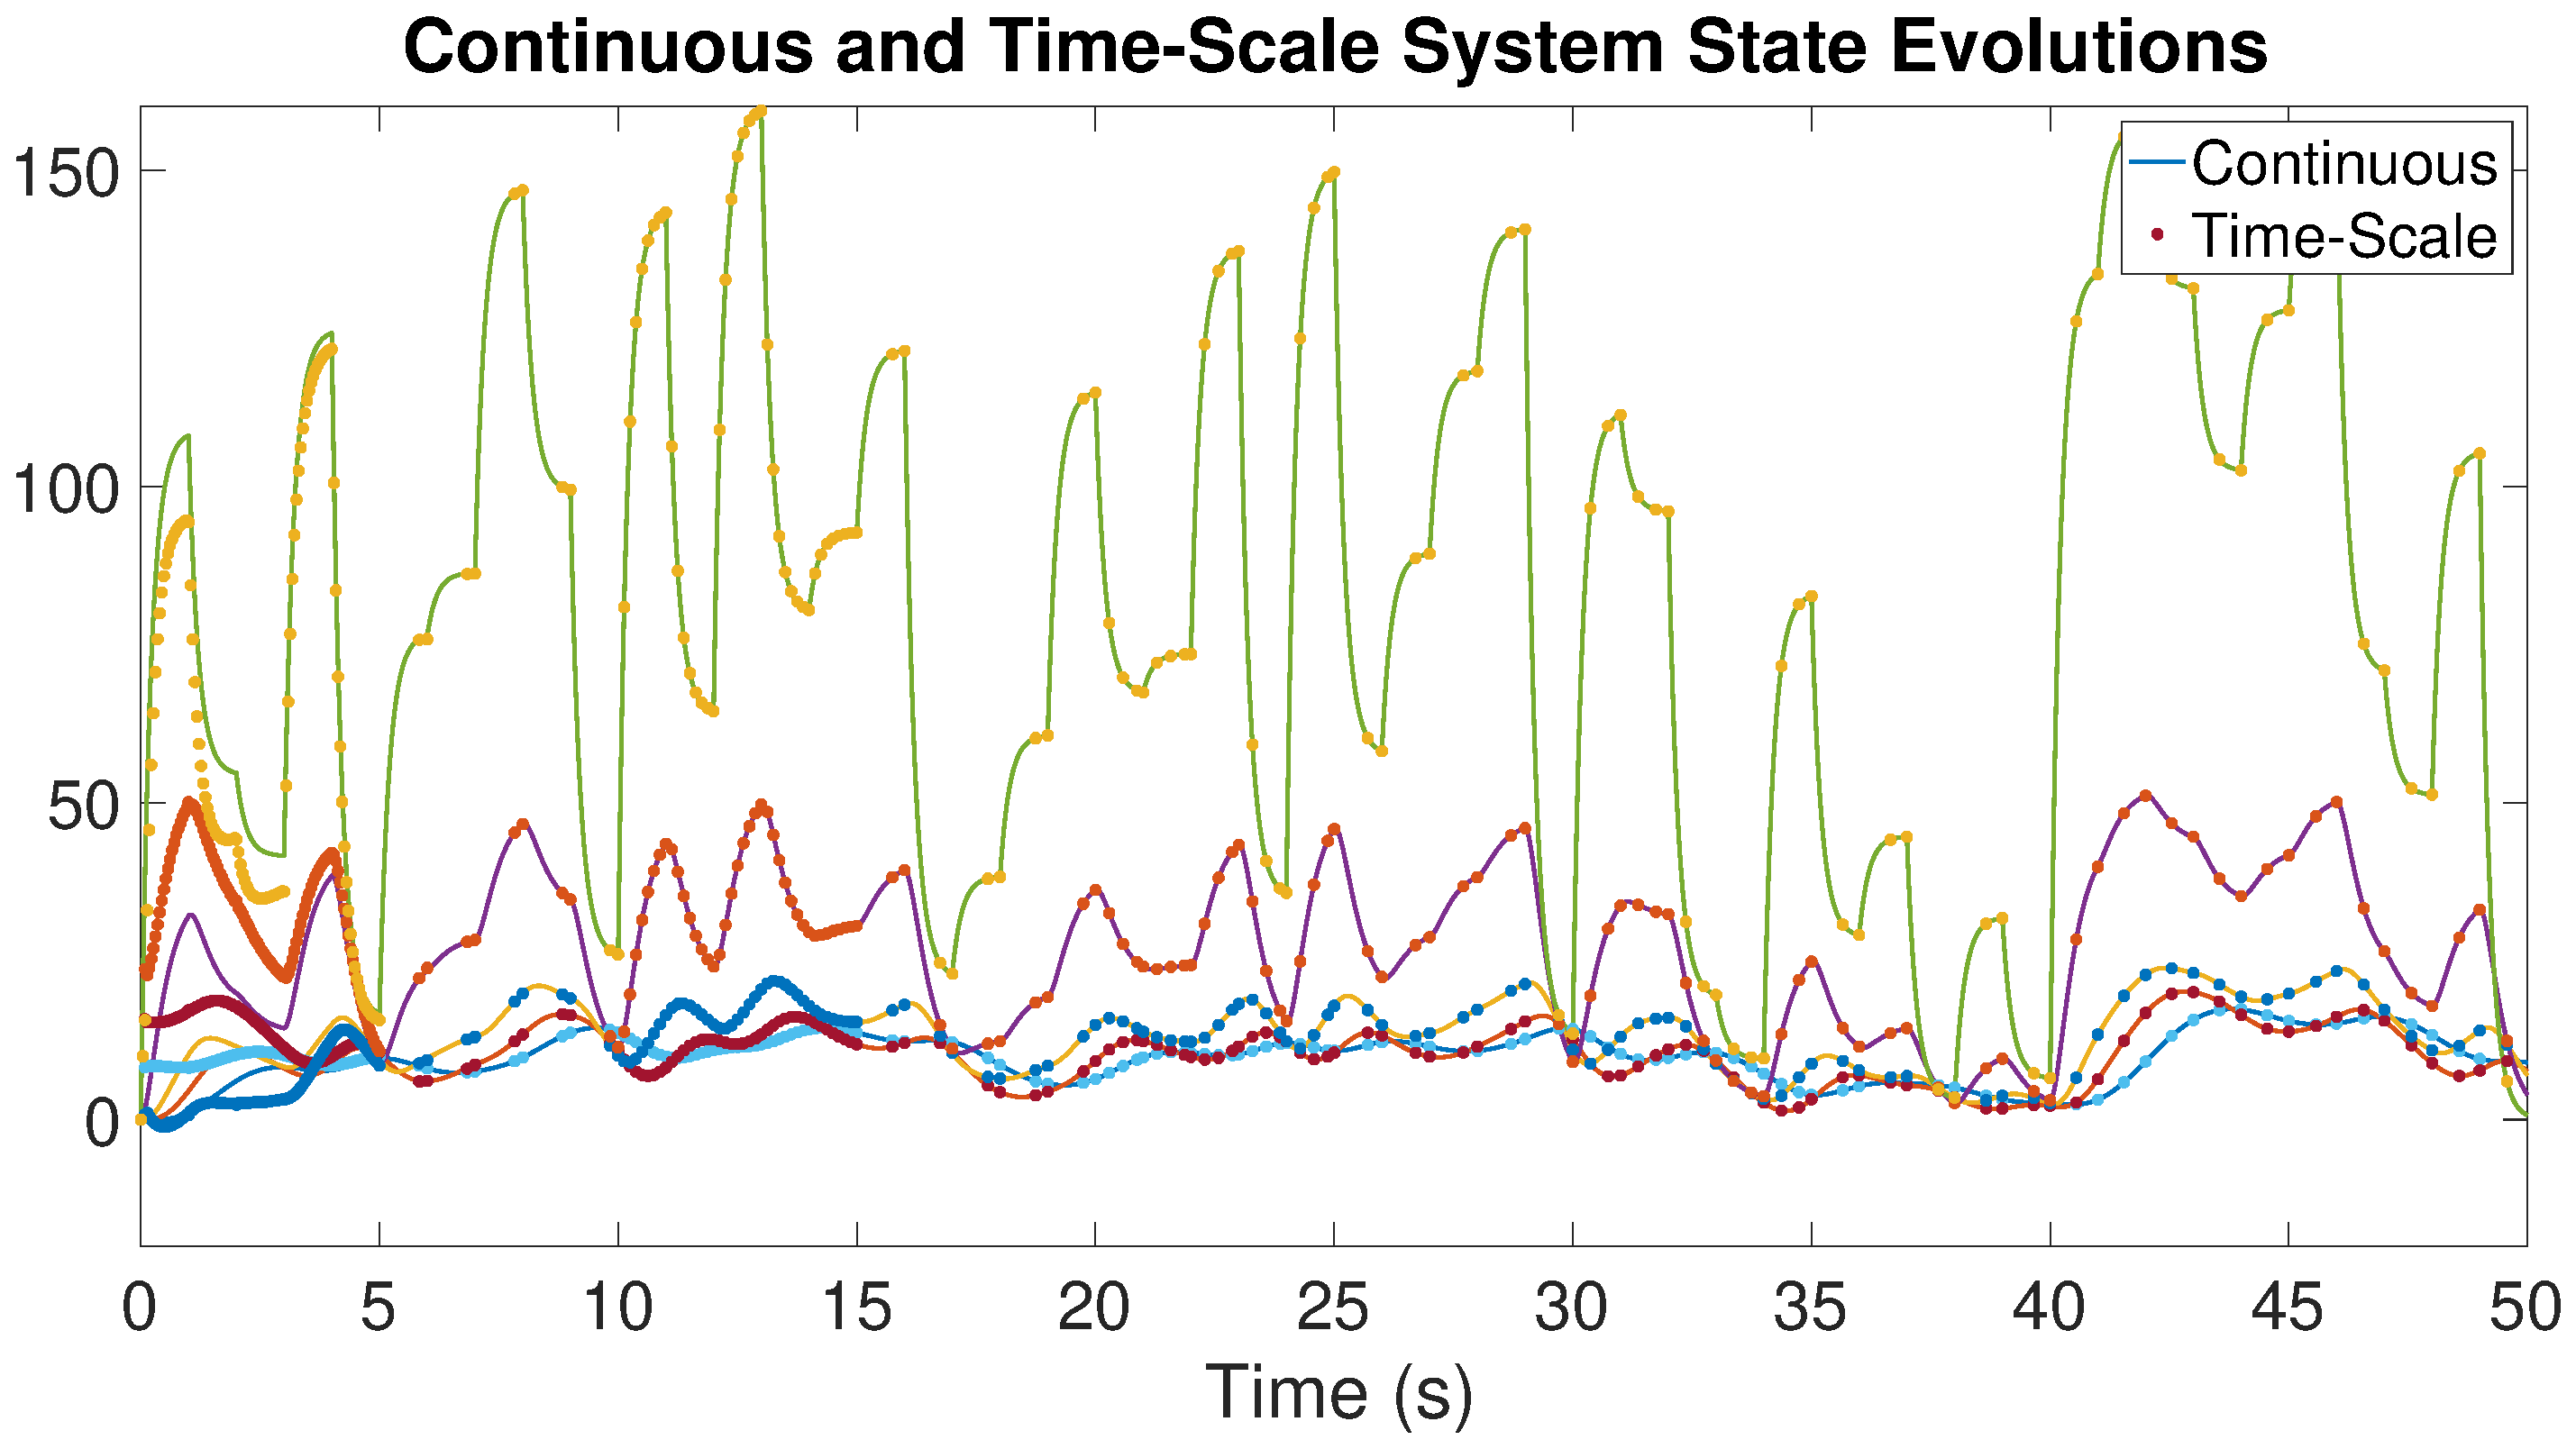
\includegraphics[width=\linewidth]{stair-input}
        \caption{Observed and system's states.}%
      \end{figure}
    \end{column}%
    \hfill%
    \begin{column}{0.55\textwidth}
      \begin{figure}[ht!]
        \centering
        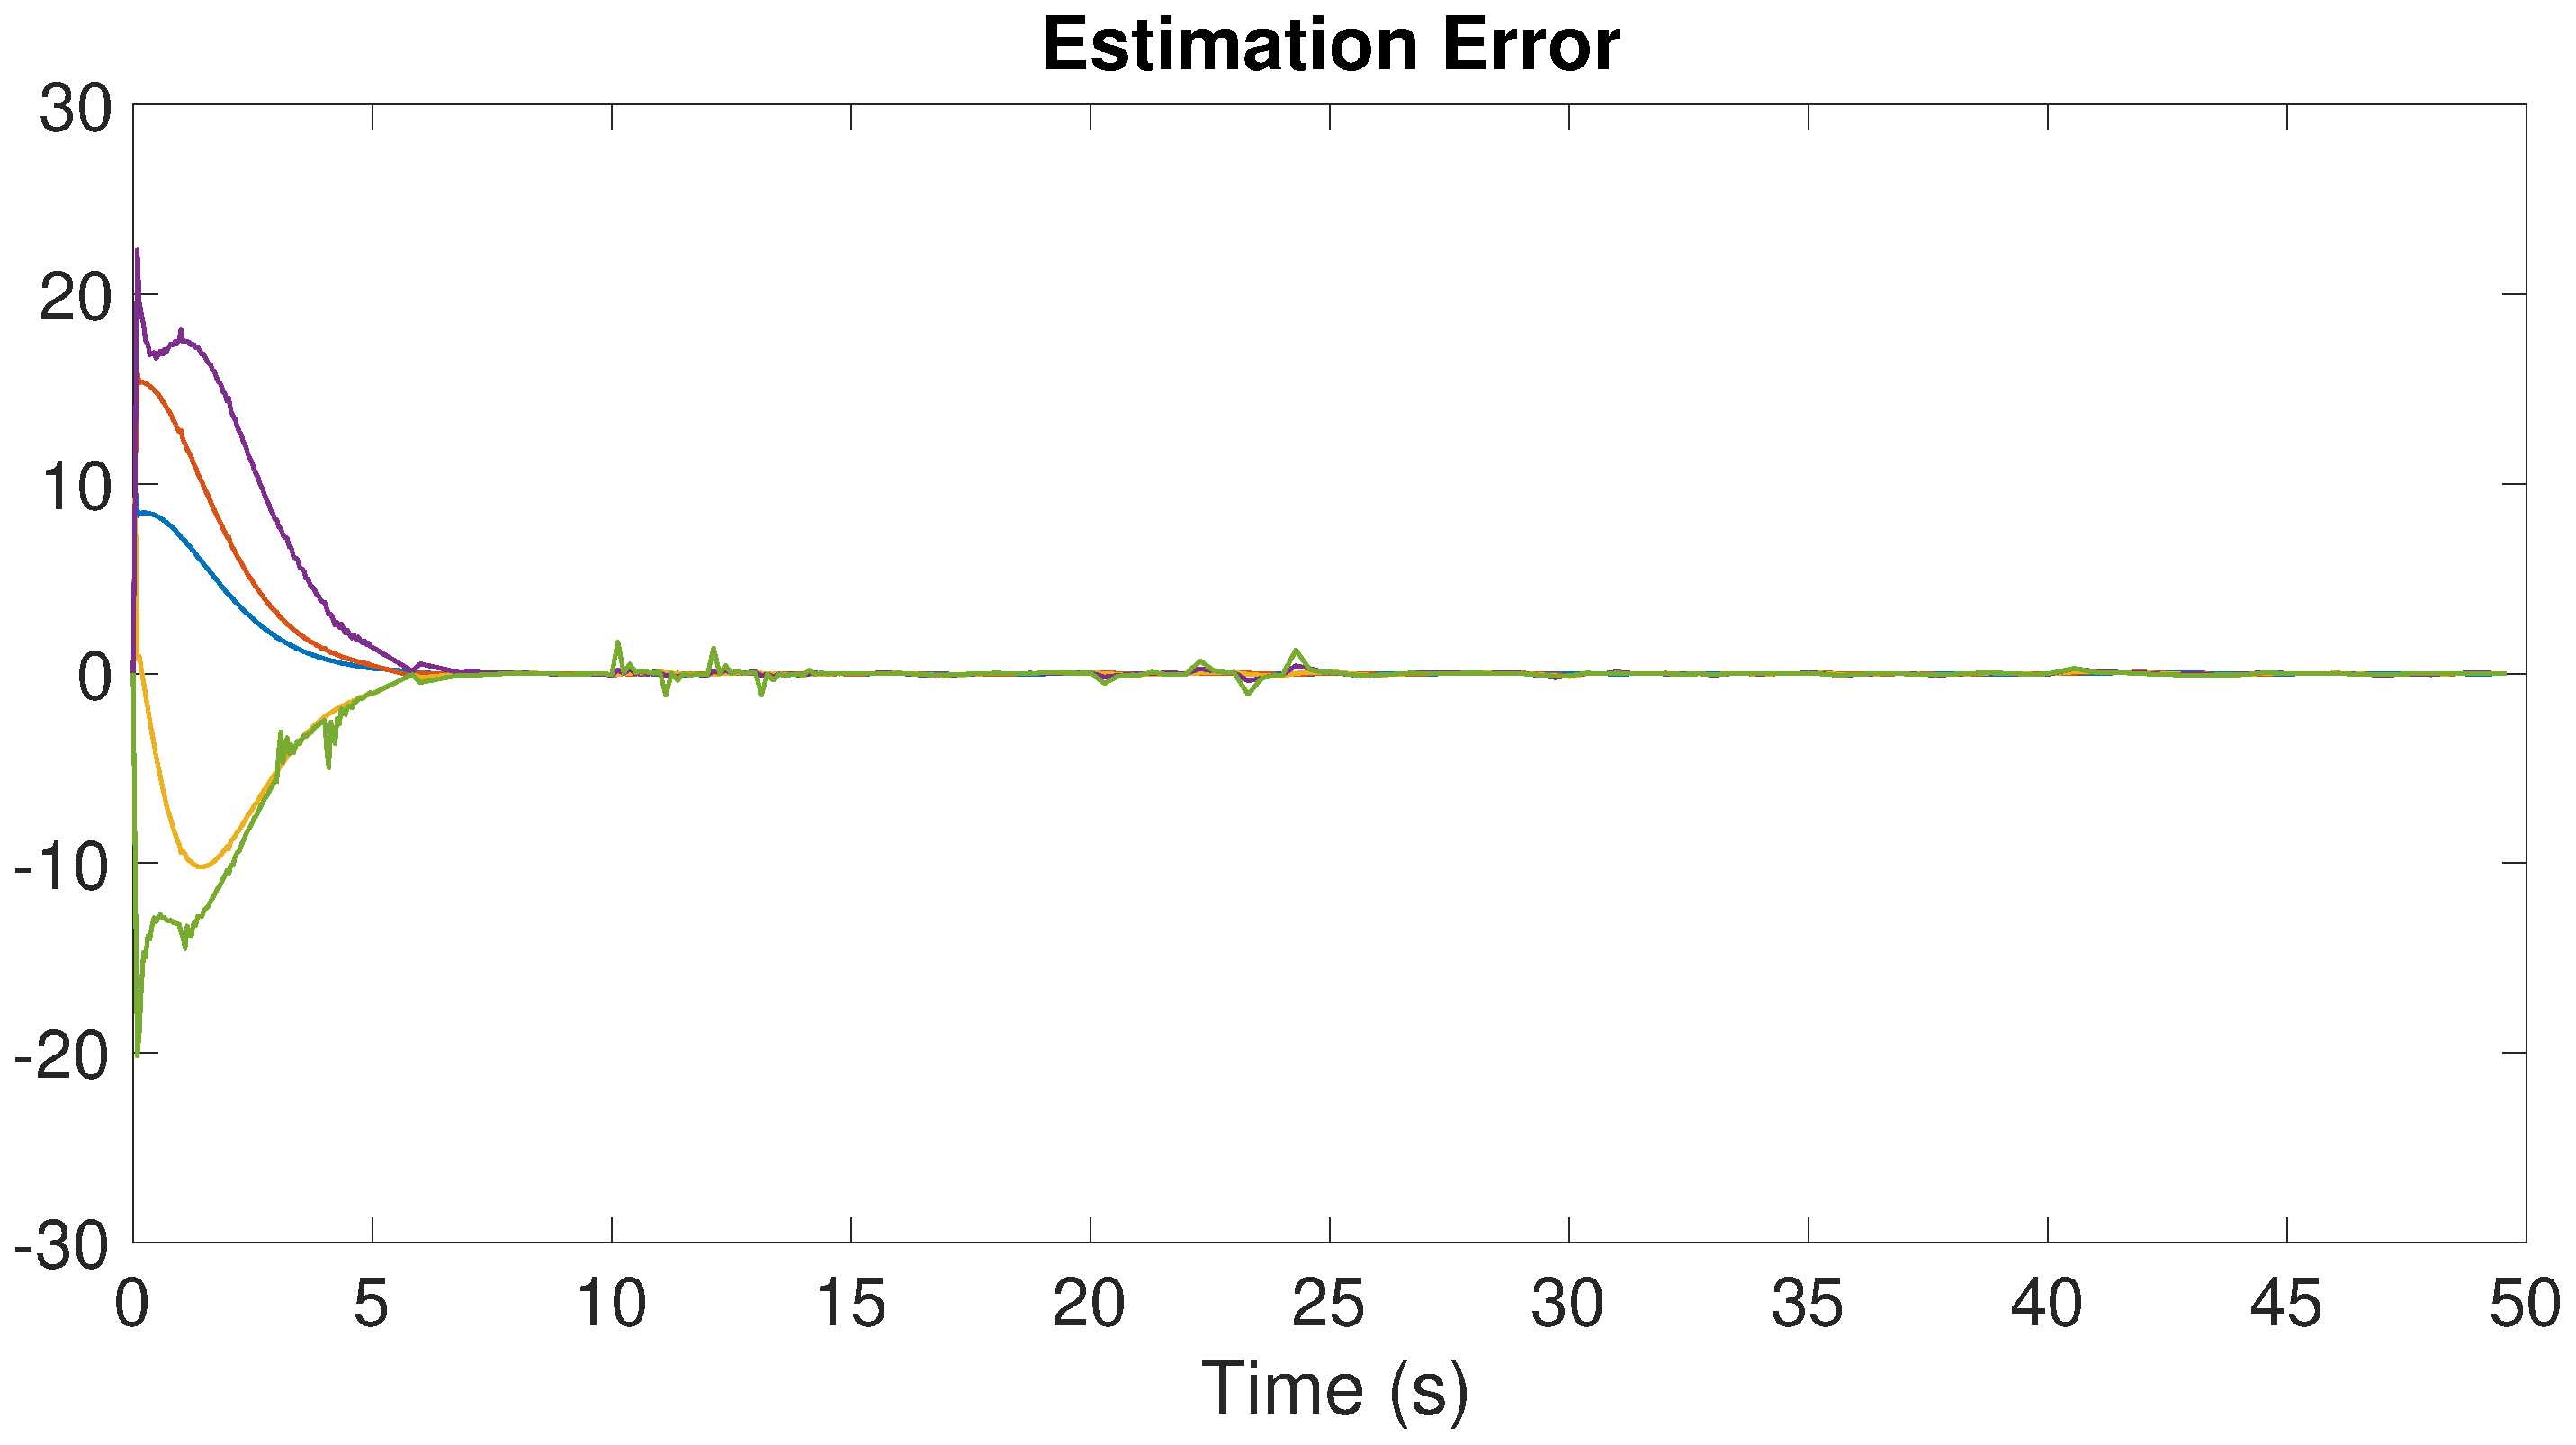
\includegraphics[width=\linewidth]{stair-input-error}
        \caption{Estimation error.}%
      \end{figure}
    \end{column}%
  \end{columns}
\end{slide}

\begin{slide}{Results}
  \begin{columns}[c]
    \begin{column}{0.55\textwidth}
      \begin{figure}[ht!]
        \centering
        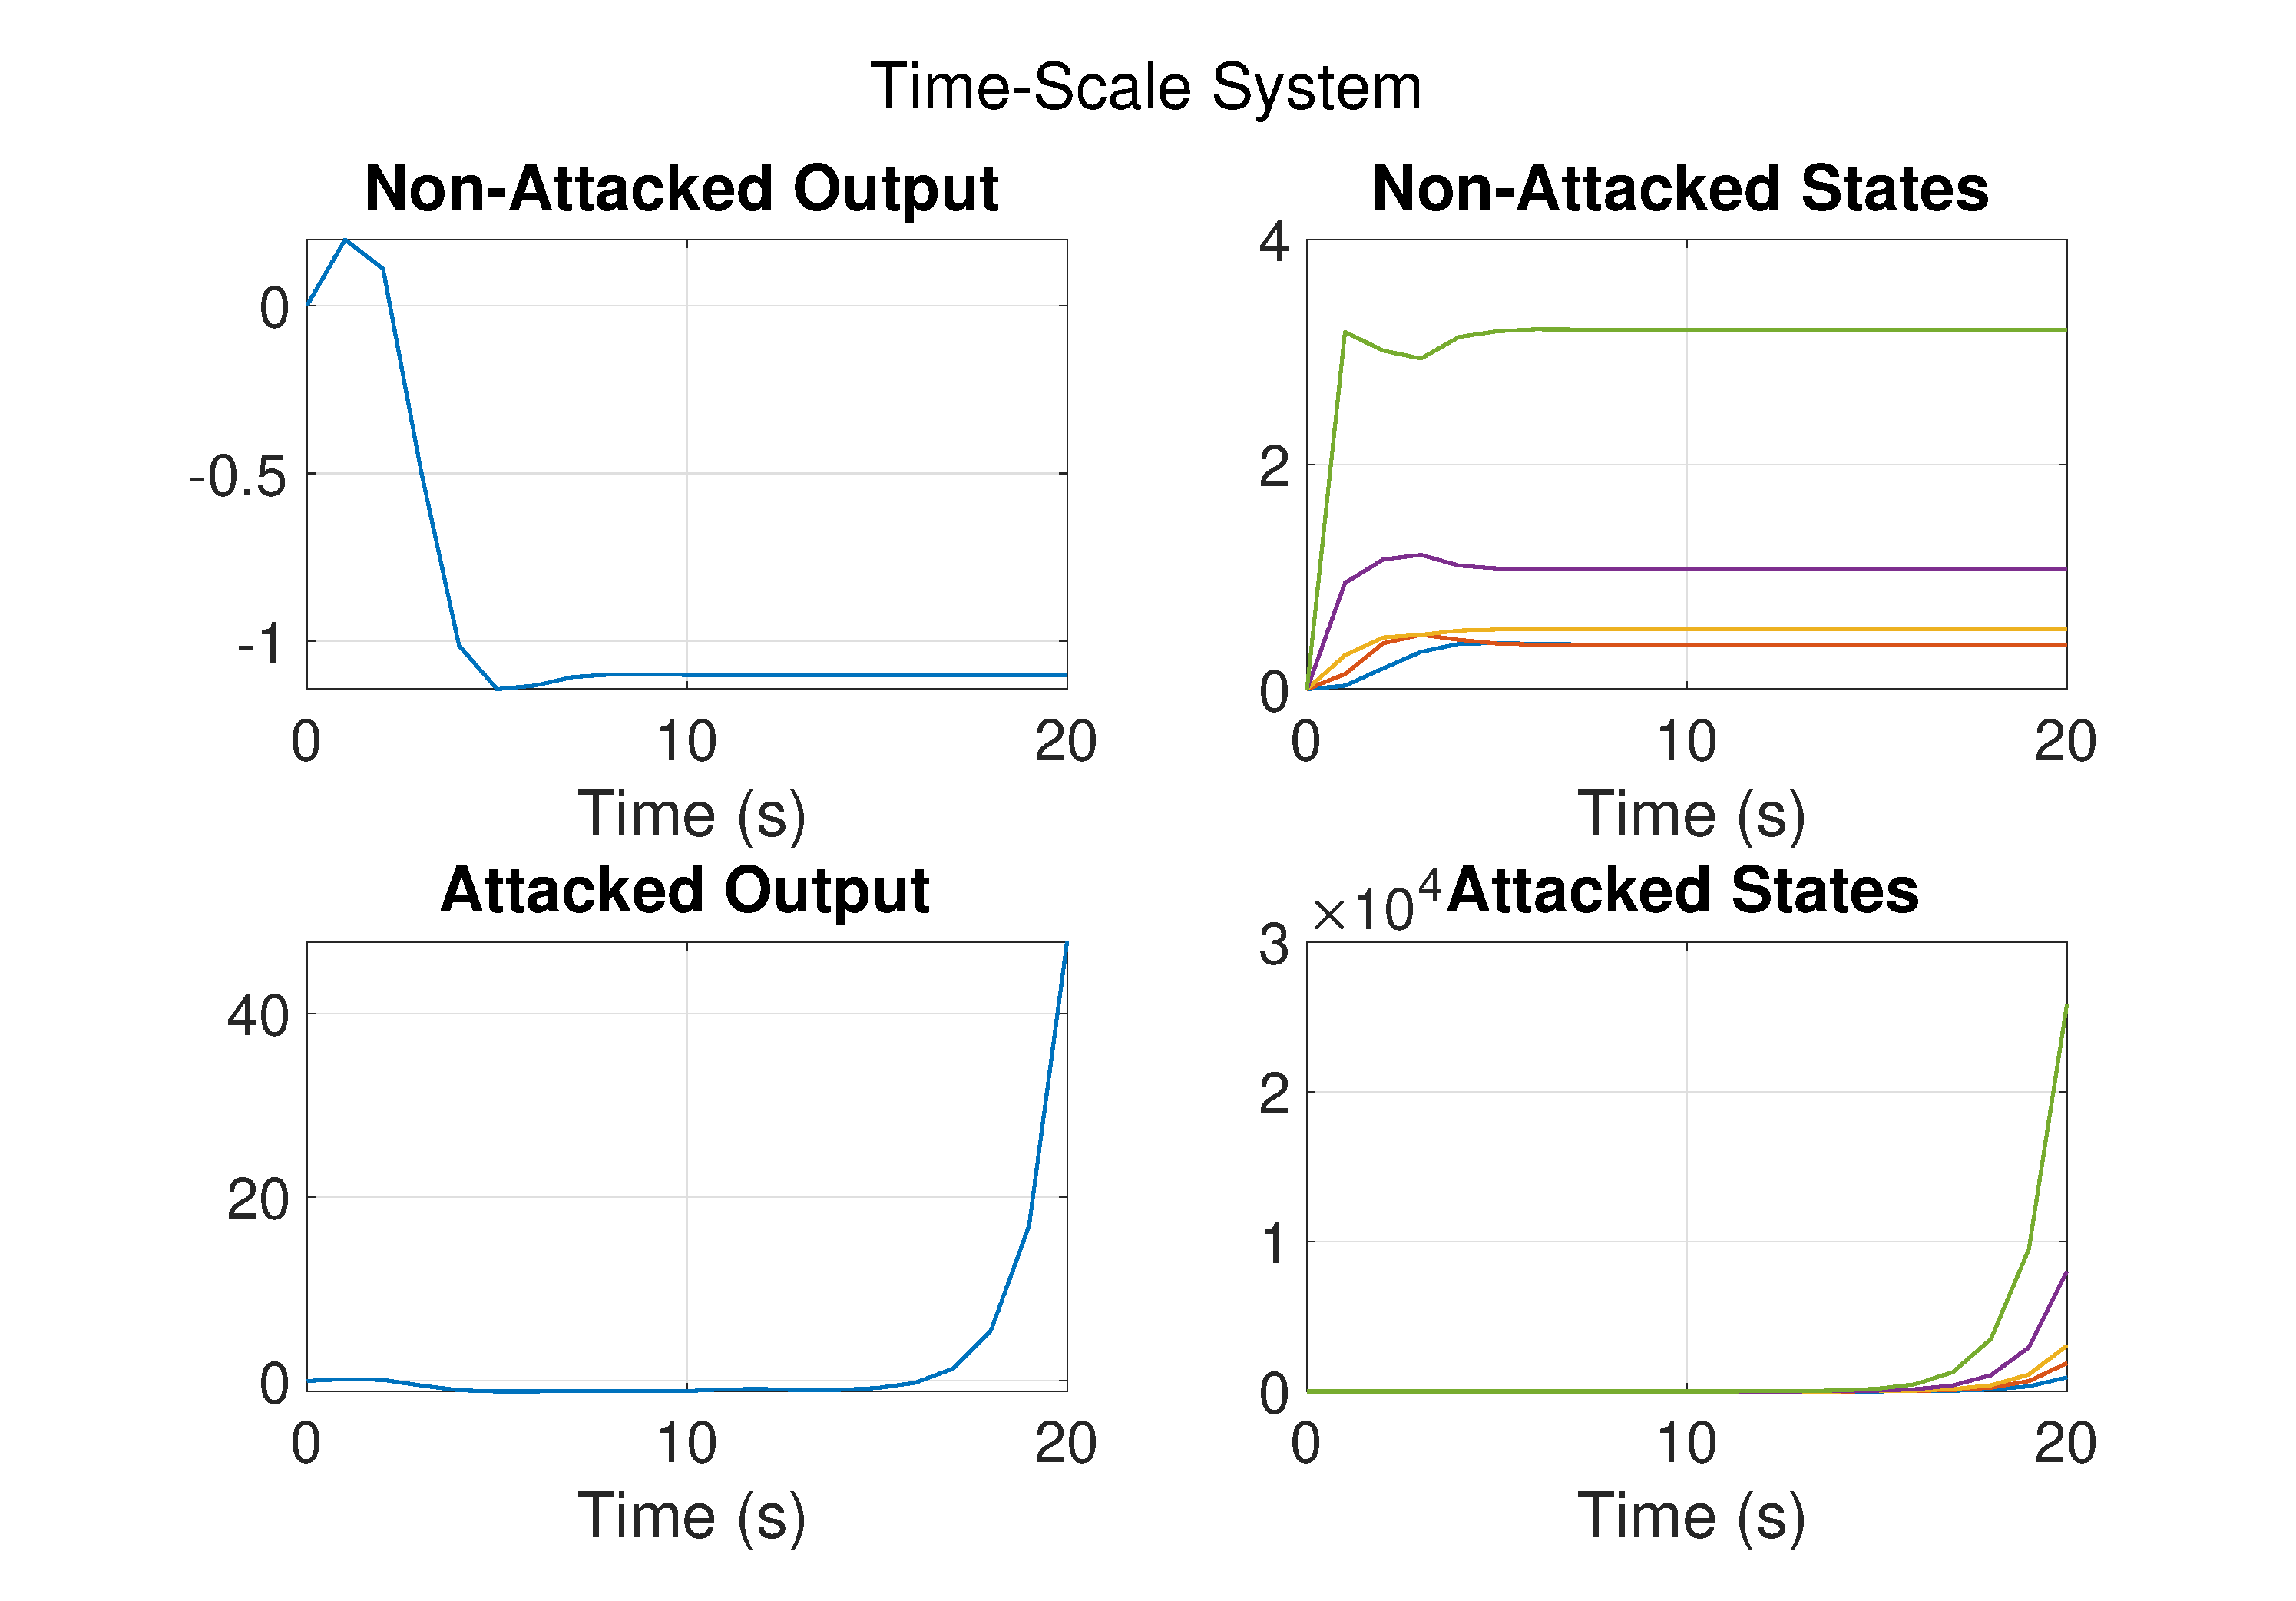
\includegraphics[width=\linewidth]{ts-system}
        \caption{Time-scale system's observer with \(\mu=\SI{1}{\second}\).}%
      \end{figure}
    \end{column}%
    \hfill%
    \begin{column}{0.55\textwidth}
      \begin{figure}[ht!]
        \centering
        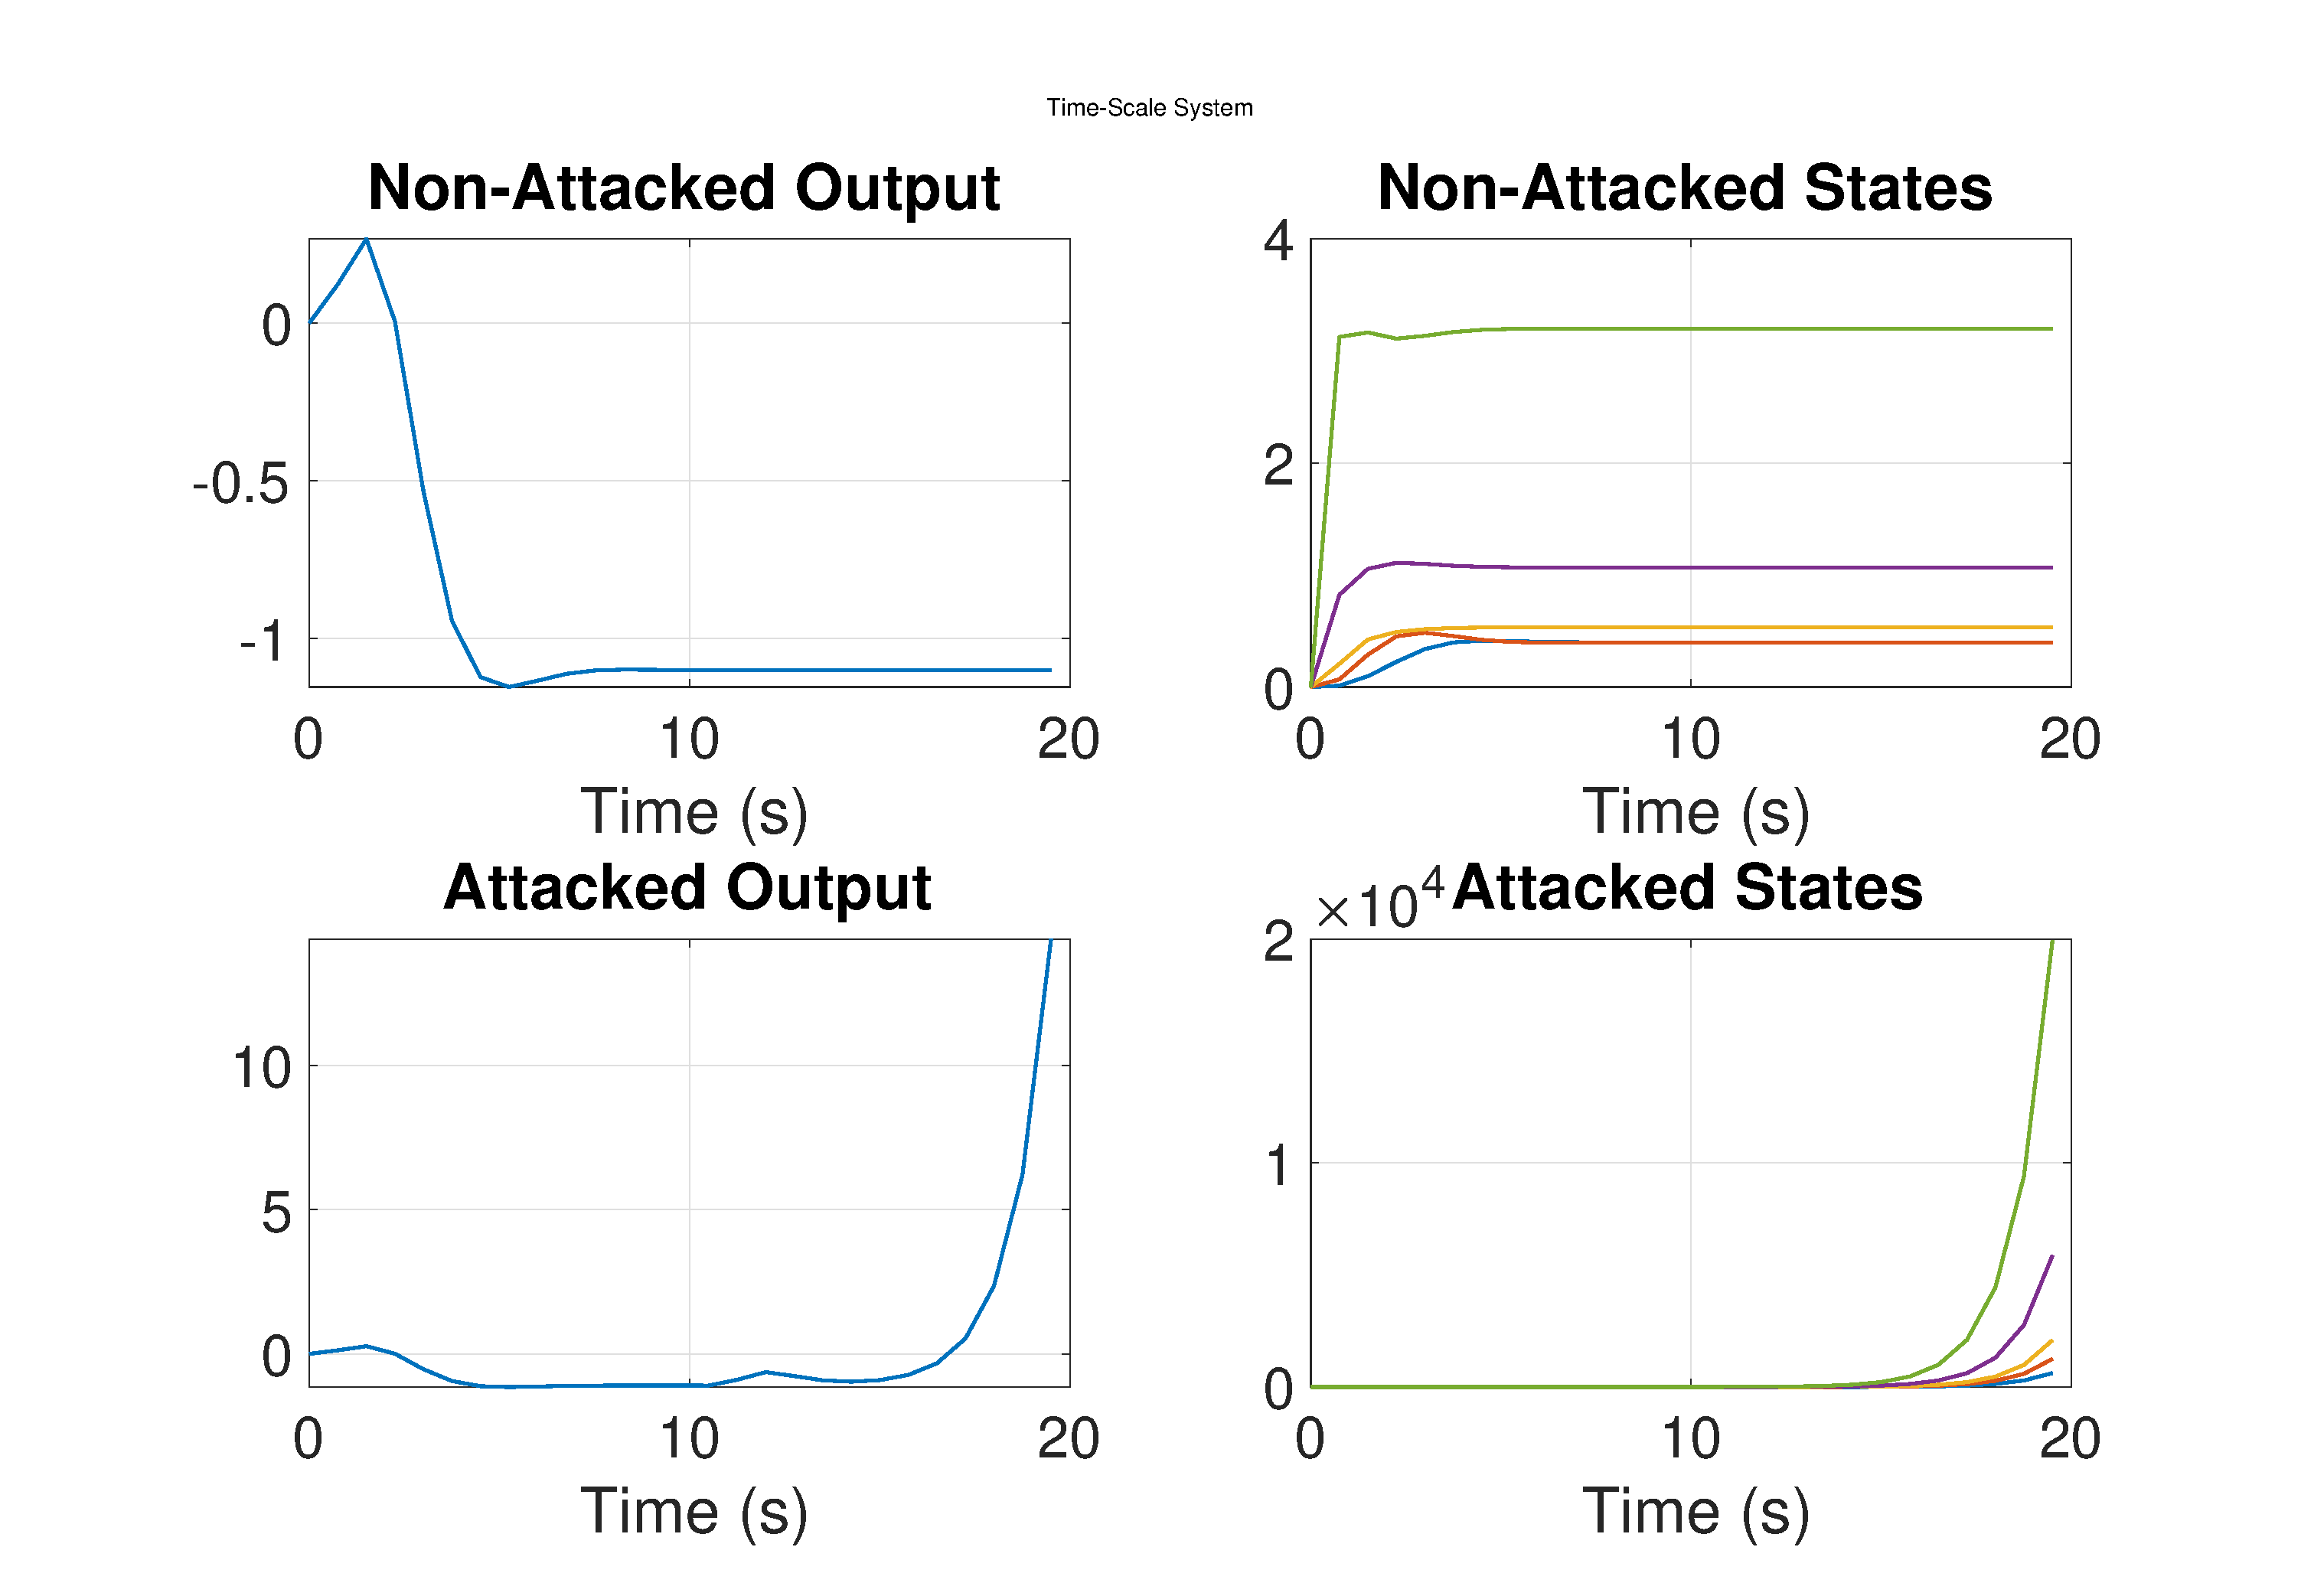
\includegraphics[width=\linewidth]{ts-system2}
        \caption{Time-scale system's observer with \(\mu=\SI{0.75}{\second}\).}%
      \end{figure}
    \end{column}%
  \end{columns}
\end{slide}


\begin{frame}[allowframebreaks]{Referências}
  \nocite{*}
  \printbibliography{}
\end{frame}
\end{document}
